\documentclass[12pt,a4paper]{report}
\usepackage[french]{babel}
\usepackage[T1]{fontenc}
\usepackage[utf8]{inputenc}
\usepackage{minitoc}
\usepackage{graphicx}
\usepackage{multicol}
\usepackage{epigraph}
\usepackage{xcolor}
\usepackage{enumitem} % Personalisation des listes
\usepackage[ruled,vlined]{algorithm2e}
\usepackage{amsmath}
\usepackage{array}
\usepackage{pdfpages}
\newcommand{\Mod}[1]{\ (\mathrm{mod}\ #1)}
\SetAlFnt{\small}
\SetAlCapFnt{\large}
\SetAlCapNameFnt{\large}
\usepackage{algorithmic}
\usepackage{tabularx}
\usepackage{biblatex}
\addbibresource{biblio.bib}


\algsetup{linenosize=\tiny}

\setcounter{secnumdepth}{3}
\setcounter{tocdepth}{1}
\setcounter{minitocdepth}{3}

\begin{document}
    
%Wow je crée une couverture dans un fichier différent comme ça si je modifie la couverture le reste ne sera pas modifié :)



\begin{titlepage}
    \centering
    {\bfseries\large
        Telecom Nancy\\
        Université de Lorraine\\
        Groupe 21\\
        \vskip1cm
        Flavien Ledeux \\
Guilhèm Roura \\
Céline Zhu \\
    }    
    \vfill
        {\bfseries\Huge
        PROJET PPII\\
    }   
    \vfill{}
    
\includegraphics[width=5cm]{logo_TNCY.png}
    \vfill{}
        {\bfseries\Large
      Sébastien Da Silva \\
Gérald Oster
    } 
    \vfill
    {\bfseries\Large
        Villers-lès-Nancy\\
        Avril 2021\\
    }   
\end{titlepage}
\chapter*{Introduction}

\epigraph{\itshape“We don't just build websites, we build websites that SELLS”}{
― Christopher Dayagdag}
\begin{multicols}{3}
Le concours Mines-Telecom, en raison du nombre de participants et d'épreuves, comporte de nombreuses données différentes. Cela nécessite donc des outils adaptés afin de pouvoir les vérifier, les traiter et les exploiter.

Afin de pouvoir stocker ces données, il faut de plus avoir une base de données adaptée, que l'on pourra remplir avec les données issues de ce concours.

Ainsi, il nous a été demandé pour ce projet de concevoir une base de données devant conserver l'ensemble des données du concours. Mais il a aussi été demandé de concevoir et réaliser une application permettant de remplir et d'exploiter cette base de données. Le remplissage doit pouvoir être fait à partir de fichiers Excel comportant des données issues du concours.

Le but précis de cette application est, à partir des fichiers Excel, de remplir la base de données. De plus, l'application doit permettre de retrouver les données selon divers critères ou filtres.

Une certaine liberté est laissée sur la conception de l'application et de la base de données, la seul contrainte étant d'utiliser au moins un des 3 langages imposés (C, Python, Java) pour l'application.
\end{multicols}
\dominitoc
\tableofcontents
\chapter{État de l'art}


\section{Technologies utilisable pour le projet }
 \minitoc
\subsection{Présentation des SGBD (système de gestion de base de données) considérés}

\subsubsection{SQLite :} 

SQLite est un SGBD utilisant le langage SQL.
La base de données consiste en un fichier dans lequel toutes les informations sont stockées.
En plus de son incorporation trivial dans un projet, le SGBD ne demande pas beaucoup de mémoire.
Enfin, tous les membres du groupe ont utilisé SQLite au cours des TPs de WeBD.
\cite{SQLite-wiki} \cite{sqlite}

\subsubsection{MySQL :}

MySQL est un SGBD utilisant le langage SQL.
La base de données est située sur un serveur. Pour consulter des informations, il faut être connecté en réseau avec le serveur dans lequel la base est hébergée.
Cela demande donc la configuration d’un serveur qui doit héberger la base de données tout au long du projet ainsi que de pallier aux problèmes de serveur introuvable et de connexion non sécurisée.
Enfin, tous les membres du groupe n'ont pas d’expérience avec MySQL.
\cite{MySQL-wiki}


\subsection{Présentation des frameworks considérés}

\subsubsection{Flask :} 

Flask est un framework permettant de développer des sites internet grâce à sa génération de pages HTML.
Le framework est basé sur Python, langage que nous avons vu ou revu au cours du premier semestre. De plus, ce framework est facile à prendre en main car il possède moins de fonctionnalité que les frameworks standards.
D’autre part, Flask intègre directement la gestion de SQLite.
Enfin, Flask est utilisé dans le cadre du module WEBD, dans lequel nous avons pu nous initier à son utilisation.
\cite{Flask}


\subsubsection{JavaFX :}

JavaFX est un framework permettant de développer des interfaces graphiques pour des applications bureautiques.
Le framework est basé sur Java, langage que nous avons vu ou revu au cours du deuxième semestre lors de nos cours de programmation orientée objet (OOP).
JavaFX n’intègre pas de gestion de SGBD. Cette fonction est déléguée à d'autres APIs à installer en plus du framework.
Enfin, tous les membres du groupe n'ont pas d’expérience avec ce framework.
\cite{JavaFX-wiki}

\subsubsection{Qt :}

Qt est un framework permettant de développer des interfaces graphiques pour des applications bureautiques.
Le framework est basé sur du C++, langage que nous n’avons pas vu en cours mais qui ressemble à du C orienté objet. Le langage C a cependant été vu en cours.
Qt intègre la gestion d’un grand nombre de SGBD. Cependant, en fonction du SGBD choisi, il se peut qu'il soit nécessaire de compiler Qt.
Enfin, aucun membre du groupe n'a d’expérience avec ce framework.
\cite{Qt}

\subsection{Conclusion}

Nous avons décidé de choisir le MySQL comme SGBD car ce dernier fonctionne en local et qu’il ne demande pas la mise en place d’un serveur, que nous aurions dû hébergé à nos frais.

Le framework Qt a été exclu d’emblée car nous n’avions pas assez d’expérience dans son utilisation, malgré sa grande variété d’outils pour se connecter à des SGBD.
D’autre part, JavaFX a été aussi exclu en faveur de Flask car ce dernier n'intègre pas directement les outils pour se connecter au SGBD que nous avons choisi.

Ainsi, nous avons choisi d’utiliser pour le projet SQLite et Flask de part leur aisance d’utilisation quand ces derniers sont utilisés en conjonction.


\chapter{Conception et mise en œuvre d’une base de données relationnelle}
\minitoc
Le sujet nous demandait de créer une base de données sous forme normal 3 (3FN), puis de dé-normaliser si cela était voulu ou nécessaire. Dans un premier temps nous présenterons les 3 formes normales obligatoire du sujet. Ensuite nous expliqueront nos choix de conception.

\section{Normalisation}
Les formes normales des bases de données sont définies récursivement, c'est a dire qu'une forme plus évolué de normalisation dépend des formes plus basses. Ainsi la forme 3FN dépend de la forme 2FN qui dépend elle même de la forme 1FN, normalisation la plus basse des bases de données.
\cite{Database_normalization-wiki}

\subsection{1FN} :
La forme 1FN correspond à l'atomicité des informations de la base de données. C'est à dire que chaque élément de la base contient au plus une donnée. Cela nous empêche donc d'avoir des listes d'éléments dans une entrée de la base de données

\subsection{2FN}
La forme 2FN correspond, en plus de la norme 1FN, au principe d'avoir chaque élément d'une table ne dépendant que de sa ou ses clés primaires. C'est-à-dire qu'un élément, pour être dans la même table que la clé primaire, doit uniquement dépendre de cette dernière ou d'éléments dépendant de cette dernière, et si elle dépend partiellement de cette dernière, alors une nouvelle table doit être créé avec une combinaison de plusieurs clés étrangères comme clé primaire. 

\subsection{3FN}
La forme 3FN correspond, en plus de la norme 2FN, au principe de retirer la transitivité des dépendances au seins d'une même table. C'est-à-dire que si un élément A dépend de B et que B dépend C alors A ne peut pas être dans la même table que C. Nous devons donc avoir deux tables, une où A dépend de B et une autre où B dépend de C.

\subsection{Autre pratique}
Un principe courant dans les bases de données est de donner des codes à des données qui n'en possèdent pas dans le jeu sur lequel notre modèle se base. Cela permet d'économiser de la mémoire en évitant de stocker des informations redondantes en entière à l'aide de chaînes de caractères mais de leur assigner une valeur bien moins gourmande, généralement un entier, pour les représenter. Cependant cela à pour conséquence, dans certains cas, d'augmenter le temps des requêtes. 

\section{Choix de conception}
Concrètement, nous avons centré notre schéma autour d'une table \textit{candidat}, pour laquelle chaque entrée représente un candidat. Cette table comporte donc de nombreux attributs, puisqu'elle contient les informations sur les candidats fourni par le fichier \textit{Inscription}.
Nous y avons aussi ajouté des données liés au candidats, mais obtenu ou extrapolé depuis d'autre fichier.
La grande majorité des attributs reprennent des colonnes du fichier inscription.
Cependant, afin d'éviter la redondance et d'être normale, si le fichier "Inscription" contenant un code et le libellé associé, alors la table "candidat" ne contient que le code.
De même, pour des données répétées, tel que la qualité du candidat (Boursier/Pupille) ou encore un nom de pays ou de ville, la table contient alors un entier qui référence cette donnée.

Ces données répétées se trouvent dans des tables auxiliaires, contenant en clé primaire le code associé, et en autre attribut le libellé de la donnée.

Enfin, il y a des tables auxiliaires qui contiennent plusieurs données, par exemple celles pour les établissements.
\chapter{Composants logiciels informatiques}
 \minitoc
\section{Script}
\subsection{Script python}
\subsubsection{BDDCreation}
Ce script permet de créer une base de données depuis à l’aide d’un fichier texte qui liste les différentes tables, le tout noté au format SQL. \\
La script prend deux arguments :
\begin{itemize}
    \item \textbf{file\_path} : le chemin vers le fichiers qui contient le code SQL
    \item \textbf{database\_path} : le chemin où la base de données sera créé
\end{itemize} 

Le script prend aussi en compte les commentaires SQL placé dans le fichier texte. Ces dernier doivent être marqué par la chaîne de caractère suivante : ‘//’.\\
Le script prend prend aussi en compte le cas ou le chemin du la futur base de données est déjà occupé par un autre fichier. Dans ce cas, le script laisse la main à l'utilisateur pour choisir s' il veut continuer le script et ainsi supprimer le fichier problématique.

Le script requiert l'extension python click pour fonctionner.


\subsubsection{ImportRepository}
Ce script permet d'insérer les données de tous les fichiers présents dans un répertoire vers une base de données.
Le script prend deux arguments : 
\begin{itemize}
    \item \textbf{repository\_path} : le chemin vers le répertoire où sont stocké les fichiers
    \item \textbf{database\_path} : le chemin de la base de données qui va subir l’opération
\end{itemize}
Le script prend uniquement en compte les fichiers directement présents dans le répertoire, c'est-à-dire que les fichiers présents dans un répertoire situé dans le répertoire passé en paramètre seront ignorés.

Dans un premier temps, le script récupère le chemin de tous les fichiers.\\
Une fois les fichiers récupérés, le script va chercher une chaîne de caractères clés (\ref{tab:TableKeyChar} page \pageref{tab:TableKeyChar}) dans leur nom pour sélectionner la méthode de traitement approprié. Si un fichier ne contient aucune chaîne de caractères clé, il sera ignoré.\\
Enfin, le script exécute la méthode de traitement associée à chaque fichier retenu.

Comme le temps du script est proportionnel à la quantité de données à insérer dans la base de données, un indicateur est affiché pour permettre à l'utilisateur d'avoir une idée de la progression du script.

Le script requiert l'extension python click pour fonctionner.


\begin{table}[]
    \centering
    \begin{tabularx}{\linewidth}{ | X | X | X | }
      \hline
            description  &  mot clé associé / type & exemple de fichier du jeu de test\\
      \hline
            liste des écoles & listeecoles & listeEcoles.xlsx\\
      \hline
            liste des établissement & listeetablissement & listeEtablissements .xlsx\\
      \hline
            liste des états possible d'un voeux & listeetatsreponsesappel & listeEtatsReponses Appel.xlsx\\
      \hline
            liste des personnes inscrites & inscription & Inscription.xlsx\\
      \hline
            liste des informations de multiples candidats admissibles & admissible\_ & ADMISSIBLE \_ATS.xlsx\\
      \hline
          liste des informations d'un candidat lié à sa classe  & classes\_ & Classes\_MP\_CMT \_spe\_XXXX.xlsx \\
      \hline
          liste des informations d'un candidat lié à son code scei & scei & Classes\_MP\_CMT \_spe\_XXXX \_SCEI.csv\\
      \hline
          liste des information d'un candidat et de son rang écrit  & ecrit\_ & Ecrit\_MP.xlsx\\
      \hline
          liste des information d'un candidat et de son rang oral & oral\_ & Oral\_MP.xlsx\\
      \hline
          liste des informations de multiples candidats admis & admis\_ & ADMIS\_ATS.xlsx\\
      \hline
          liste des voeux de multiples candidats & listevoeux\_ & listeVoeux\_ATS.xlsx\\
      \hline
          liste des résultats des oraux CMT de multiples candidats & cmt\_oraux & CMT\_Oraux \_YYYY\_MP.xlsx\\
      \hline
          liste des résultats ecrit de multiples candidats & resultatecrit\_ & ResultatEcrit\_DD \_MM\_YYYY \_ATS.xlsx\\
      \hline
          liste des résultats oraux de multiples candidats & resultatoral\_ & ResultatOral\_DD \_MM\_YYYY \_ATS.xlsx\\
      \hline
    \end{tabularx}
    \caption{\textit{Tableau des chaînes de caractères clées}} 
    \label{tab:TableKeyChar}
\end{table}

\subsection{Autre Script}
\subsubsection{installer}
    Le script Installer, disponicle en .bat(Windows) et en .sh(linux) détecte si Python3 est installé sur l'ordinateur. Si Python3 n'est pas installé le script l'installe. Ensuite le script crée un environnement virtuel nommé ProjectEnvironnement où les dépenses du projet seront installées.\\
    La version Linux fonctionne avec les distributions possédant les gestionnaires de package suivant : DPKG, DNF, et YUM.

\section{Traitement des fichiers}

\subsection{Lecture des fichiers}
Le lecture des fichiers s'effectue à l'aide de la fonction ReadFile du fichier PolyMorph\_Lecture.
Cette fonction renvoie une liste dont le première élément est le nom du fichier ouvert, et tous les éléments suivant étant les lignes du fichier. Les lignes sont modélisé par une liste où chaque case de la ligne correspond a une information trouvé sur la ligne.

La lecture des fichiers a été implémenter avec le polymorphisme en tête. Ce concept de programmation orienté objet consiste a créer un classe interface qui définie les entêtes fonctions pour être sur que toutes les classes qui implémente cette interface utilisent la même syntaxe. Ainsi, nous avons 3 classes définie :
\begin{itemize}
    \item FileReading : la classe interface
    \item XLRS : la classe qui gère les fichiers .xlrs
    \item CSV : la classe qui gère les fichiers .csv
\end{itemize}
Cela permet au projet d'évoluer plus simplement au cours du temps si il faut ajouter une nouvelle extension a traité ou de devoir placer les données de la base de données dans un fichiers d'une extension géré.

Dans un premier temps, la fonction vérifie si le fichier existe. Ensuite, elle va regarder l'extension du fichier pour connaître son type. Dans notre cas, seul deux types de fichier sont autorisés : .xlsx et .csv.
La fonction va appeler la méthode read de la classe adéquate pour obtenir les données. Si cette méthode n'existe pas, alors la fonction s'arrête. Enfin, la fonction retourne la liste contenant le nom du fichiers et les données.

\subsubsection{Lecture de fichier tableur}

La lecture des fichiers se base sur 2 modules python:

\begin{itemize}
    \item \textbf{openpyxl} : Pour la lecture des fichiers .xslx
    \item \textbf{csv} (standard) : Pour la lecture des fichiers .csv
\end{itemize}

Ceci permet l'ouverture et la lecture de fichier .xlsx et .csv, ce qui couvre tous les formats de fichier attendus pour les fichiers de données.

\subsection{Fonction d'insertion des données}

\subsubsection{Fonction Uploadnotes}


Cette fonction prend deux arguments : les données d'un fichier obtenue préalablement à l'aide de la fonction ReadFile et d'une chaîne de caractères  correspondant au type d'examen passé. La fonctions est a utiliser avec les fichiers  de types "resultatoral\_", "resultatecrit\_" et "cmt\_oraux"(\ref{tab:TableKeyChar} page \pageref{tab:TableKeyChar}).
La fonction a pour but d'ajouter des notes ainsi que d'autres informations relatifs aux notes tel que le nom du jury dans la table \textit{notes} ainsi que dans que dans deux autres tables lié : \textit{matiere} et \textit{typeExam}.

La fonctions appel n-1 fois la fonction AddMatiere, avec n étant le nombre de données sur la première ligne, pour ajouter à la base de données les différentes matières et avoir leur code.
La fonction AddTypeExam est aussi appelé pour ajouté un type d'examen et obtenir son code.
Enfin, pour chaque donnée de chaque ligne, on associe dans la base de données, la note ou valeur à un candidats, une matière et un type d'examen en utilisant leur code.

\subsubsection{Fonction UploadEcole}


Cette fonction prend en unique argument les données d'un fichier obtenue préalablement à l'aide de la fonction ReadFile. Ce fichier doit être du type de "listeecoles" (\ref{tab:TableKeyChar} page \pageref{tab:TableKeyChar})
La fonction a pour but d'ajouter de multiples écoles à la base de données dans la tables \textit{ecole}.
Pour chaque ligne du fichier, on ajoute le nom de l'école ainsi que son code dans la base de données.

\subsubsection{Fonction UploadOralEcrit}


Cette fonction prend deux arguments : les données d'un fichier obtenue préalablement à l'aide de la fonction ReadFile et d'une chaîne de caractères  correspondant au type d'examen associé au rang, c'est à dire soit oral, soit écrit. La fonctions est a utiliser avec les fichiers  de types "oral\_", "ecrit\_" (\ref{tab:TableKeyChar} page \pageref{tab:TableKeyChar}).
La fonction a pour but d'ajouter des candidats ainsi que d'autres informations relatifs a ces derniers dans la tables \textit{candidats} ainsi que dans que dans les table : \textit{pays}, \textit{commune}, \textit{civilite}, \textit{voie}, \textit{matiere}, \textit{typeExam} et \textit{notes}.


Dans un premier temps, la fonction trouve la filière associé aux candidats à l'aide du nom du fichier de provenance.
Pour chaque ligne nous appelons les fonctions AddCommune, AddCountry pour obtenir enregistrer différentes informations lié au candidats et en obtenir leur code pour y faire référence.
Ensuite, nous ajoutons un nouveau candidat dans la tables \textit{candidat} ou nous le mettons a jour si il existe en utilisant les données de la ligne et des codes des communes, des pays et des civilités.
Enfin, nous ajoutons son rang dans la tables \textit{notes} à  l'aide du code du candidats, du type d'examen, et de la matière rang créé spécialement.

\subsubsection{Fonction UploadAdm}


Cette fonction prend deux arguments : les données d'un fichier obtenue préalablement à l'aide de la fonction ReadFile et d'une chaîne de caractères  correspondant au type du candidat, c'est à dire soit admissible, soit admis. La fonctions est a utiliser avec les fichiers  de types "admis\_", "admissible\_" (\ref{tab:TableKeyChar} page \pageref{tab:TableKeyChar}).
La fonction a pour but d'ajouter des candidats ainsi que d'autres informations relatifs a ces derniers dans la tables \textit{candidats} ainsi que dans que dans les table : \textit{pays}, \textit{commune}, \textit{civilite}, \textit{voie}, \textit{resultat}.

Dans un premier temps, la fonction trouve la filière associé aux candidats à l'aide du nom du fichier de provenance.
Ensuite, la fonction, à l'aide du nom du fichier dont provienne les données, regarde si les liste des candidats est de type spécifique ou non et utilise la fonction AddResultat pour obtenir le code du résultat correspondant.
Pour chaque ligne nous appelons les fonctions AddCommune, Addcountry, pour obtenir enregistrer différentes informations lié au candidats et en obtenir leur code pour y faire référence.
Ensuite, nous ajoutons un nouveau candidat dans la tables \textit{candidat} ou nous le mettons a jour si il existe en utilisant les données de la ligne et des codes des communes, des pays, des résultats et des civilités.

\subsubsection{Fonction UploadListVoeux}


Cette fonction prend en unique argument les données d'un fichier obtenue préalablement à l'aide de la fonction ReadFile. Ce fichier doit être du type de "listevoeux\_" (\ref{tab:TableKeyChar} page \pageref{tab:TableKeyChar})
La fonction a pour but d'ajouter de multiples voeux provenant de multiples candidats à la base de données dans la tables \textit{voeux\_ecole}.
Pour chaque ligne du fichier, on associe à un candidat, une école et un entier correspondant l'ordre du voeux un rang et le statuts du voeux .

\subsubsection{Fonction UploadListReponse}


Cette fonction prend en unique argument les données d'un fichier obtenue préalablement à l'aide de la fonction ReadFile. Ce fichier doit être du type de "listeetatsreponsesappel" (\ref{tab:TableKeyChar} page \pageref{tab:TableKeyChar})
La fonction a pour but d'ajouter les possibles réponses à un voeux à la base de données dans la tables \textit{reponse}.
Pour chaque ligne du fichier, on associe à un code à ce à quoi il correspond.


\subsubsection{Fonction UploadSCEI}


Cette fonction prend en unique argument les données d'un fichier obtenue préalablement à l'aide de la fonction ReadFile. Ce fichier doit être du type de "scei" (\ref{tab:TableKeyChar} page \pageref{tab:TableKeyChar})
La fonction a pour but d'ajouter d'associer a un candidat des informations gràce a son rang dans sa filière en modifiant les tables \textit{ranginfo}, \textit{notes}, \textit{typeExam} et \textit{matiere}.
Pour chaque ligne du fichier, on associe à un rang et à une filière de multiples information. Ensuite, si un candidat de cette filière et avec ce rang existe, on ajoute le total de point qu'il a reçu lors de épreuve oral à l'aide des méthodes Add et du code candidat trouvé.


\subsubsection{Fonction UploadClasse}


Cette fonction prend deux arguments : les données d'un fichier obtenue préalablement à l'aide de la fonction ReadFile et d'une chaîne de caractères  correspondant au type du candidat, c'est à dire soit admissible, soit admis. La fonctions est a utiliser avec les fichiers  de types "admis\_", "admissible\_" (\ref{tab:TableKeyChar} page \pageref{tab:TableKeyChar}).
La fonction a pour but d'ajouter des candidats ainsi que d'autres informations relatifs a ces derniers dans la tables \textit{candidats} ainsi que dans que dans les table : \textit{pays}, \textit{commune}, \textit{civilite}, \textit{voie}, \textit{resultat}.

Dans un premier temps, la fonction trouve la filière associé aux candidats à l'aide du nom du fichier de provenance.
Ensuite, la fonctions appel n fois la fonction AddMatiere, avec n étant le nombre de matières présentes sur la première ligne, pour ajouter à la base de données les différentes matières et avoir leur code.
La fonction AddResultat est aussi appelé pour obtenir les codes des résultats associable au candidats du ficher. De même on appel la fonction AddExamType pour obtenir le code pour l'examen oral et l'examen écrit.

Dans un second temps, pour chaque ligne, nous appelons les fonctions AddCommune, AddCountry, AddVoie, pour obtenir enregistrer différentes informations lié au candidats et en obtenir leur code pour y faire référence.
Ensuite, nous ajoutons un nouveau candidat dans la tables \textit{candidat} ou nous le mettons a jour si il existe en utilisant les données de la ligne et des codes des communes, des pays, des résultats et des civilités. Puis, nous ajoutons dans la table \textit{notes} les notes du candidat associé à la ligne


\subsubsection{Fonction UploadEtabli}

Cette fonction permet d'ajouter les données un fichier de la forme de "listeEtablissement"

Elle prend pour unique paramètre le fichier sous forme de liste, obtenu avec la fonction ReadFile.


Pour chaque ligne du fichier excel, elle crée un dictionnaire correspondant à l'entrée que l'on veut ajouter dans la base de donnée. Pour cela, on fait une première requête basé sur le RNE de l'établissement, pour tester si l'établissement à déjà été ajouté. Il a en effet pu avoir été ajouté précédemment depuis le fichier "Inscription". Dans ce cas certains champs seront non renseigné.

Si l'établissement est déjà présent, on met à jour tous les champs avec la valeur venant de "listeEtablissement".

Autrement, on ajoute une nouvelle entrée correspondant à l'établissement.


\subsubsection{Fonction UploadInscription}


Cette fonction prend \textbf{en unique argument} un fichier sous forme d'une liste, obtenu par une des fonctions de lecture de fichier.
Ce fichier doit \textbf{être du type} de \textit{Inscription} ((\ref{tab:TableKeyChar} page \pageref{tab:TableKeyChar}).
Elle a pour but de remplir la grande majorité de attributs de la table \textit{candidat}, ainsi que différentes tables auxiliaires, notamment celles liées directement à la table candidat.


Cette fonction va parcourir chaque ligne pour à chaque fois faire les insertion nécessaire suivant la ligne lu.

Pour une ligne, \textbf{elle appelle d'abord une dizaine de fonction \textit{Add[...]}}.
Ces dernières permettent d'ajouter la donnée à une table auxiliaire, et renvoient l'identifiant associé pour la référencer.
Si la donnée se trouvais déjà dans la table, elle donne l'identifiant sans avoir fait d'insertion.


Ensuite, un dictionnaire correspondant à la table \textit{candidat} est rempli. La clé correspond au nom de l'attribut, et la valeur correspond à la valeur associé.
Ce dictionnaire comprends ainsi la quasi totalité des attributs de \textit{candidat}.


Pour chaque valeur, il y a \textbf{trois possibilités}:
\begin{itemize}
    \item la valeur du fichier est \textbf{inséré tel quel}. Cela correspond notamment aux valeurs entière ne nécessitant pas de traitement, où aux valeurs unique (ou presque) comme l'adresse
    \item \textbf{La valeur est transformé}, au moyen d'une \textbf{fonction de traitement}, puis insérez. Cela correspond en particulier aux numéro de téléphone, qui sont formatés autant que possible sous un même format
	\item La valeur rentrée est \textbf{l'identifiant référençant la vrai valeur} dans une autre table. C'est l'identifiant obtenu plus tôt avec les fonctions \textit{Add[...]}
\end{itemize}


Enfin, à partir du dictionnaire, les données sont inséré ou mise à jour, suivant qu'un entrée pour ce numéro de candidat existe déjà ou pas.
Cette insertion/mise à jour est faite au moyen de la fonction d'ajout \textit{InsertOrUpdateData}

%Les 2 paragraphes suivant (commentés) sont potentiellement invalide si on peut garder la connection en passant le "cur" en paramètre

%SQLite ne permet pas d'ouvrir la connections avec la base de donnée dans une fonction, puis de la ré ouvrir dans une autre fonction auquel on fait appel. Les fonctions "Add[...]" font appel à la base de donnée, on ne peut donc pas l'appeler alors que la base de donnée à été ouverte. IL faut ainsi l'ouvrir, commit les changements puis la fermé pour chaque ligne.


%En terme de performance temporel, la fonction a été mesuré à 5min30 pour un fichier Inscription.xslx complet de 15 000 candidats. Cela semble acceptable puisque c'est un coût unique, la problématique de temps se posant principalement lors de l'accès à la base de donnée, et non lors de l'insertion. De plus, il n'est pas attendu qu'un grand nombre de fichier "Inscription" soit ajouté à la base de donnée.

\subsubsection{Fonction InsertData / InsertOrUpdateData}

Ces 2 fonctions sont assez semblables, \textit{InsertOrUpdateData} n'étant qu'une version augmentée de \textit{InsertData}

\textbf{InsertData}


Cette fonction à pour but de généraliser l'ajout de données dans une table. Elle prend \textbf{4 paramètres} et \textbf{1 valeur de retour}:

\begin{itemize}
    \item \textbf{param1 = data :} C'est le paramètre principal de la fonction, un dictionnaire contenant toutes les données qui seront éventuellement ajoutées 
    \item \textbf{param2 = name\_id:} C'est le nom de l'attribut qui sera renvoyé à la fin. Il s'agit de la valeur permettant de référencer l'entrée depuis une autre table 
    \item \textbf{param3 = name\_table:} C'est le nom de la table dans laquelle faire l'insertion
    \item \textbf{param4 = name\_select:} C'est le nom de l'attribut qui sera utilisé pour vérifier si l'entrée existe déjà ou pas
    \item \textbf{retour:} La valeur associée à l'attribut name\_id
\end{itemize}


Le paramètre \textit{data} est un \textbf{dictionnaire} contenant l'entrée à ajouter.
Chaque couple clé/valeur est un attribut à remplir dans la table.
La \textit{clé} est le nom de l'attribut dans la base de donnée, et la \textit{valeur} est la valeur de l'attribut pour cette entrée.


La fonction va ouvrir la connexion avec la base de donnée et faire une première requête. Celle-ce essaye de récupérer la valeur de l'attribut \textit{name\_id} pour l'entrée dont la valeur de l'attribut \textit{name\_select} coïncide avec la valeur passé en paramètre.
Si on a un résultat, l'entrée existe déjà, et on ferme la connexion. On renvoie alors la valeur de \textit{name\_id} obtenu.

Si la première requête ne donne rien, alors l'entrée n'existe pas encore. On va alors, avec le dictionnaire et le nom de la table, effectuer une requête qui va ajouter l'entrée.
On effectue alors une 3ème requête, identique à la première, afin de récupérer la valeur de l'attribut \textit{name\_id}, qui sera alors la valeur renvoyée.

\textbf{InsertOrUpdateData}

Cette fonction a les même paramètres et valeur de retour, et est quasi identique. Cependant, si la première requête nous renvoie une résultat, alors au lieu de ne rien faire on va insérer les données en remplaçant éventuellement celle qui était déjà présentent. On ne fait cependant pas de 3ème requête et on renvoie la valeur obtenu dès le départ.


L'intérêt de cette deuxième fonction est d'éviter des requêtes et des changement de valeurs inutiles, dans le cas où on sait que si l'entrée existe déjà, alors il n'y a rien à rajouter.


\subsubsection{Fonction AddXXXX}

Les fonctions de la formes \textit{Add[...]} sont toutes très courtes, puisqu'elles se basent principalement sur la fonction \textit{InsertData}.

Elles sont chacune lié à une table, et permettent d'insérer un ou plusieurs attributs.

\textbf{Paramètre(s) :} le ou les attributs à insérer. Certain paramètres peuvent être optionnels.

\textbf{Retourne: } l'attribut qui permet de référencer l'entrée depuis une autre table.
 
 
Ces fonctions peuvent être appelé dans 2 cas:
 
\begin{enumerate}
    \item On lit un fichier et on a obtenu une ou plusieurs donnée allant ensemble. On appelle alors la fonction pour les insérer si elles n'étaient pas déjà présentes. On peut éventuellement utiliser la valeur de retour pour référencer ces données depuis une autres table (en majorité depuis la table "candidat").
    \item On veut uniquement la valeur permettant de référencer une donnée, qu'on sait être déjà présente.
\end{enumerate}

Le principal cas où on utilise 2 paramètres est celui où l'on connais un code et son libellé associé, par exemple pour le pays. Or, le code associé à un pays n'est présent que dans le fichier Inscription, mais il y a des pays dans d'autres fichiers.


Le paramètre du numéro de code est alors optionnel, pour 2 raisons. Tout d'abord, pour pouvoir ajouter une nouveau pays si on ne connaît pas le code. Le code sera éventuellement ajouté lors d'un appel ultérieur de la fonction. En deuxième, pour pouvoir obtenir la clé primaire auto-incrémentée associée au pays en ayant uniquement à spécifier le libellé, et ce avec la même fonction.

De manière général, cette série de fonction se contente de crée un dictionnaire et d'appeler \textit{InsertData} avec les bon paramètres, puis de renvoyer sa valeurs de retour.


\subsection{Test de l'insertion}
\subsubsection{Test unitaire}
Pour tester l'exactitude de notre insertion de données, chaque fonction possède des tests unitaires. Les tests unitaires sont gérés avec la librairie pytest.
Pour nos tests unitaires, nous avons essayé d'appliquer le concept RIGHT-BICEP:
\begin{itemize}
    \item Right : notre test est il bon?
    \item B     : Les limites sont elles correctes?
    \item i     : La relation inverse est-elle possible?
    \item C     : Peut on croiser nos résultats avec des fonctions développées par des tiers?
    \item E     : Peut on forcer une erreur?
    \item P     : Les performances de la fonction sont elles acceptables? 
\end{itemize}

Bien que certaines parties du concept ne peuvent s'appliquer dans notre cas, les principes des limites et des performances ont pue être tester sur nos fonctions.

Un test standard correspond à l'insertion dans la base de données de quelques lignes d'un fichier excel compatible à la fonction. Dans ce dernier, nous essayons d'aller aux limites de nos fonctions à l'aide de notre jeux de données.
Pour vérifier que tout c'est passé comme prévue, nous effectuons un SELECT pour récupérer le jeux de données et le comparer à ce que nous aurions théoriquement du trouver.

\subsubsection{Test de cohérence}
Une première choses à noter est qu'en SQLite, bien que l'on spécifie des types pour les attributs, ces types ne sont pas nécessairement contraignants. \cite{sqlite}


Il est donc pertinent de vérifier le type des valeurs réellement enregistrées.
Par exemple que les attributs sensés contenir des entiers contiennent bien des entiers.
Cela concerne notamment les attributs qui référence une autre table via un identifiant, mais aussi les valeurs supposé entière, comme certaines date, ou encore des départements.


Il faut ensuite vérifier autant que possible que les données contenues sont celles attendues.
Par exemple, pour toutes les entrées, le champ "email" doit avoir le format d'un email.
Ce genre de vérification peut notamment être effectuée au moyen de Regex.
Dans python, cela se fait par le module standard \textit{re}.
Ce module offre des opérations sur les expressions régulières similaires aux regex Perl.\cite{module_re}
\chapter{Statistiques}
   \minitoc
      \section{Généralités}

      Dans le cadre de notre projet, nous allons effectuer quelques analyses statistiques avec l'ensemble des données fournies.
      
      Dans cette perspective nous allons clarifier quelques termes nécessaires à la bonne compréhension de notre analyse.
      \section{Analyse descriptive}
        L'analyse descriptive est un sous-domaine des méthodes quantitatives (méthodes de recherches scientifiques utilisant l'analyse mathématique et scientifique). Dans la perspective d'appliquer cette science à notre base de données, nous allons par la suite nous inspirer de la statistique descriptive, afin de caractériser différentes catégories d'élèves 

         
         \subsection{Algorithmes et explication pédagogiques}
         
         Afin de choisir les outils statistiques pertinentes aux données fournies, on s'est inspiré des données fournies par le site \textbf{www.scei-concours.fr}.
         Nous allons donc nous intéresser à l'implémentation de fonctions Python permettant le calcul de ces données ainsi que des fonctions complémentaires dont nous allons montrer l'algorithme ci-dessous.
          \begin{center}
         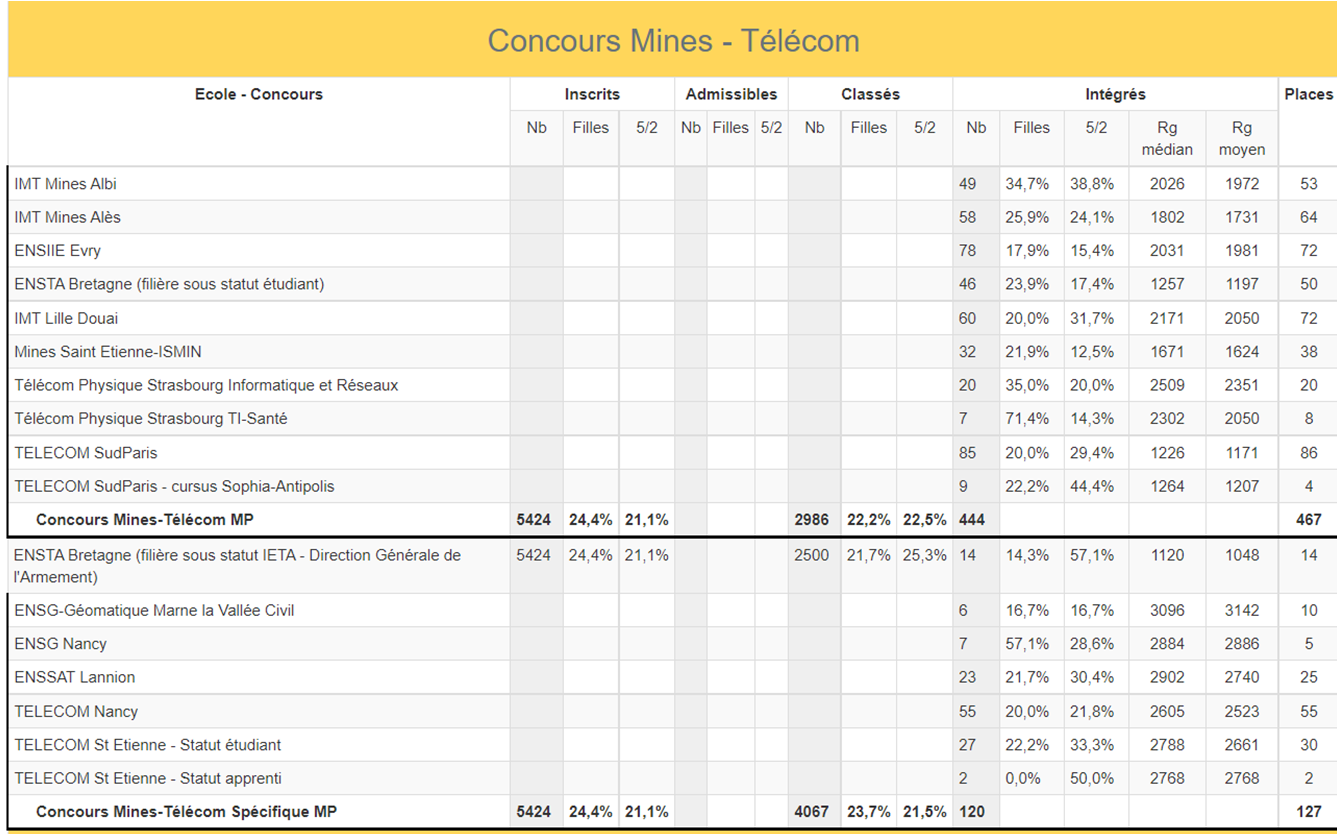
\includegraphics[width=15cm]{statimt.png}\\
         \textbf{Figure1:} Tableaux des statistiques 2020 sur scei (ici filière MP)
         \end{center}
         
         \subsubsection{Dispersion : Variance}
         La dispersion représente la variabilité des différentes valeurs que peut prendre une variable. En statistiques, il existe différentes mesures de la dispersion. Les plus courantes sont la variance, l'écart-type ou encore l'intervalle inter-quartile. C'est une mesure peu influencée par la présence de valeurs extrêmes.\\
        
        La variance est la moyenne des carrés des écarts à la moyenne:\\
        \[\sigma^2 = \frac{\displaystyle\sum_{i=1}^{n}(x_i - \mu)^2} {n} \]
        Il s'agit alors d'appliquer l'algorithme ci-dessous:\\
        
         \begin{algorithm}[H]
         \SetAlgoLined
         \KwResult{Variance}
          l=list()\;
          \For{i=0 jusqu'à la longueur de la liste l avec un pas de 1}{
           compteur=0\;
          \For{j=0 jusqu'à la longueur de la liste l avec un pas de 1}{
           \If{l(i)(j)=n}{
           compteur=compteur+1;}\
     
         }
         l=l+compteur;}
         compteur=0;\\
         \For{i=0 jusqu'à la longueur de la liste l avec un pas de 1}{
         compteur=compteur+l(i);}
         moyenne=compteur/longueur(l);\\
         compteur=0;\\
         \For{i=0 jusqu'à la longueur de la liste l avec un pas de 1}{
         compteur=compteur+($l(i)-moyenne)^2$\\ }
         Variance=compteur/longueur(l);
         
         
 \caption{Variance}
\end{algorithm}
\subsubsection{Dispersion : Ecart-type}
 L'Ecart-type est la moyenne quadratique des écarts par rapport à la moyenne ou plus simplement la racine carrée de la Variance:\\ \[\sigma = \sqrt\frac{\displaystyle\sum_{i=1}^{n}(x_i - \mu)^2} {n} \]\\
 En admettant la viabilité de l'algorithme précédent, on définie une unique instruction: l'attribution de la racine carrée de la valeur absolu du résultat obtenu par l'algorithme précédent.\\
 
        \begin{algorithm}[H]
         \SetAlgoLined
         \KwResult{Et }
          Et=$\sqrt{|Variance|}$;\;
          
 \caption{Ecart-type}
\end{algorithm}

\subsubsection{Médiane}

La médiane d'un ensemble de valeurs (échantillon, population,
distribution de probabilités) est une valeur m qui permet de couper
l'ensemble des valeurs triées en deux parties égales : mettant d'un côté
une moitié des valeurs, qui sont toutes inférieures ou égales à m et de
l'autre côté l'autre moitié des valeurs, qui sont toutes supérieures ou
égales à m (s'il y a un nombre pair de valeurs, la médiane sera la
moyenne des 2 valeurs "centrales" de la distribution): \\

    Si l'effectif total de la série est impair: $N=2p+1$, 
  la médiane est la $(p+1)^{\text{ème}}$ valeur.\;

  Si l'effectif est pair: $N=2p$, on prend en général pour médiane la
  moyenne de la $p^{\text{ème}}$ et de la $(p+1)^{\text{ème}}$ valeur. \\
  
  Il s'agit alors d'appliquer l'algorithme ci-dessous:\\

         \begin{algorithm}[H]
         \KwResult{Mediane }
          Med=list();\\
          \For{i=0 jusqu'à la longuer de la liste l avec un pas de 1}{
           med=med+liste(i)\;}
         \textbf{end}\\  
         N=entier((longueur(med)+1/2);\\
         med=sorted(med);\\
         mediane=0
         \eIf{longueur(Mediane){$\equiv 0 \mod 2$}}{mediane=med(longueur(med)+1/2)+longueur((med)-1/2)/2;}{ mediane=med(N);}
         
         \textbf{end}
         
         \caption{Mediane}
         
        \end{algorithm}
        \subsubsection{Premier Quartile}
        Les quartiles sont les 3 valeurs qui divisent les données triées en 4 parts égales, de sorte que chaque partie représente 1/4 de l'échantillon de la population. Il existe donc trois quartiles : Q1, Q2 (égal à la  médiane) et Q3. Par exemple, Q1 est la valeur telle que 25 \% des valeurs de l'échantillon lui sont inférieures, 75 \% supérieures.\\
        
         \begin{algorithm}[H]
         \KwResult{Premier Quartile }
          premquart=list();\\
          \For{i=0 jusqu'à la longueur de la liste avec un pas de 1}{
           premquart=prequart+liste(i)\;}
         \textbf{end}\\  
         N=entier((longueur(premquart))//4)\\
         premquart=sorted(premquart);\\
         Premier Quartile=0\\
         \eIf{longueur(premquart){$\equiv 0 \mod 4$}}{Premier Quartile=premquart(longueur(premquart)//4-1);}{ Premier Quartile=premquart(N);}
         
         \textbf{end}
         
         \caption{Premier Quartile}
         
        \end{algorithm}
\section{Modélisation et représentation des résultats statistiques}
Ils existent plusieurs façons de modéliser et d'exprimer les résultats des statistiques qui nous intéressent. Que ça soit des données pures organisées sous forme de tableau ou encore des cartes interactives . Nous avons décidé de garder le format scei qui semble être optimale, pour le service rendu.
\chapter{Conception et développement de l'application}
 \minitoc
 \section{Généralités}
 Le développement de l'application s'est fait principalement à partir du langage Python et du framework Flask que nous avons rencontré durant cette année scolaire dans le cadre de la WebBD et du TAPS. Le module développé présente donc deux parties: 
 \begin{itemize}
         \item La partie Front-end, c'est à dire la partie client qui permet au client d'appliquer des fonctionnalités CRUD à la base de données à partir de méthodes FORM
         \item La partie Back-end, c'est à dire la partie serveur qui gère ces modifications dans la base de données
      \end{itemize}
      Un schéma résumant l'ensemble des interactions serveur/client sera fourni à la fin de ce chapitre.\\
      
     On utilise dans cette partie un nombre de librairies Python pour parvenir à nos fins:\\
     -Flask qui permet d'utiliser le framework Flask \\
     -pdfkit qui premet de convertir des urls en pdf\\
     -sqlite3 qui permet d'accéder et de modifier la base de données en utilisant le langage SQL\\
 \section{Partie Front-end de l'application}
 La problématique du sujet nous demandais de créer une application permettant à l'utilisateur d'effectuer des requêtes (SQL ou autres) qui interagissent avec la base de données et d'en conserver le résultat sous forme HTML ou PDF.
 \subsection{Présentation de l'interface utilisateur}
 Les requêtes des utilisateurs varient grandement selon l'identité de l'utilisateur, en effet, on peut classer les profils utilisateurs dans quatre grandes catégories compte tenue de la nature des données:
\begin{itemize}
         \item Élèves qui seront intéressés uniquement par leur profil candidat
         \item Professeurs qui seront intéressés par les étudiants de leur établissement
         \item Administrateurs qui savent utiliser le SQL et veulent uploader des fichiers .xlsx ou .csv pour mettre à jour les données
         \item Curieux qui veulent tout simplement connaître des informations plus générales sur l'ensemble du concours de l'institut Mines-Télécom.
      \end{itemize}
L'objectif ici étant de permettre à tout le monde d'accéder à l'ensemble des données qui leur sont pertinentes le plus rapidement possible.
De cette manière,un utilisateur non-identifié doit alors déclarer son identité sur la page principale de l'application. Une fois identifié il se retrouvera sur une page de connexion ( à l'exception du profil "Curieux"), qui permettra à l'application de confirmer son identité en comparant les informations fournies avec celles données par la partie serveur de l'application.

FIGURE
\subsubsection{Interface Élève}
L'utilisateur "Élève" qui est identifié par son code candidat (unique) et son nom. Une fois, la connexion établie, il arrivera à sa page personnelle où il aura accès à plusieurs information:\\

\begin{itemize}
         \item Les informations personnelles le concernant tirés de la table candidat, modifiable
         \item Les notes obtenues aux écrits et aux oraux (si ces derniers ont eu lieux) 
         \item Les voeux des candidats classés dans l'ordre, modifiable

      \end{itemize}
\subsubsection{Interface Professeur}
L'utilisateur "Professeur" est identifié par le nom de son établissement ainsi le code  de son établissement "unique", il a donc accès à toutes les notes des étudiants de son établissement avec les noms et prénoms des candidats.

Logiquement les professeurs ne sont pas sensés avoir accès aux informations personnelles des étudiants
\subsubsection{Interface Administrateur}
L'utilisateur " Administrateur" est identifié par un nom et un mot de passe arbitraire qu'on a décidé pour le projet: 
\begin{itemize}
         \item nom: "Groupe21"
         \item mot de passe: "L3 M31LL3UR GR0UP3"\footnote{Les développeurs de ce projet sont conscients que le mot de passe n'est pas très sécurisé}
      \end{itemize}
      
      
Une fois la connexion établie, l'administrateur aura le choix entre trois options:
\begin{itemize}
         \item Une recherche SQL avec le schéma de la base de données en référence
         \item Une barre de recherche dynamique
         \item Une option pour ajouter et supprimer les fichiers .xls et .csv et en conséquence modifier la base de données
      \end{itemize}

\subsubsection{Interface Curieux}
Il s'agit de la visualisation des résultats des fonctions statistiques établies dans le chapitre 4. Une première visualisation des données générale sera fournie à l'utilisateur, puis des propositions plus précises seront offertes à l'utilisateur selon différents critères.
 \subsection{Architecture du Front-end}
 Cette partie est développée en Python et HTML dans le framework Flask, l'installation de nouveaux packages se fait au travers d'un environnement Python 3.0 virtuel et de la commande pip3. l'architecture du Front-end est détaillée dans la figure suivante de manière simplifiée:
  \begin{center}
         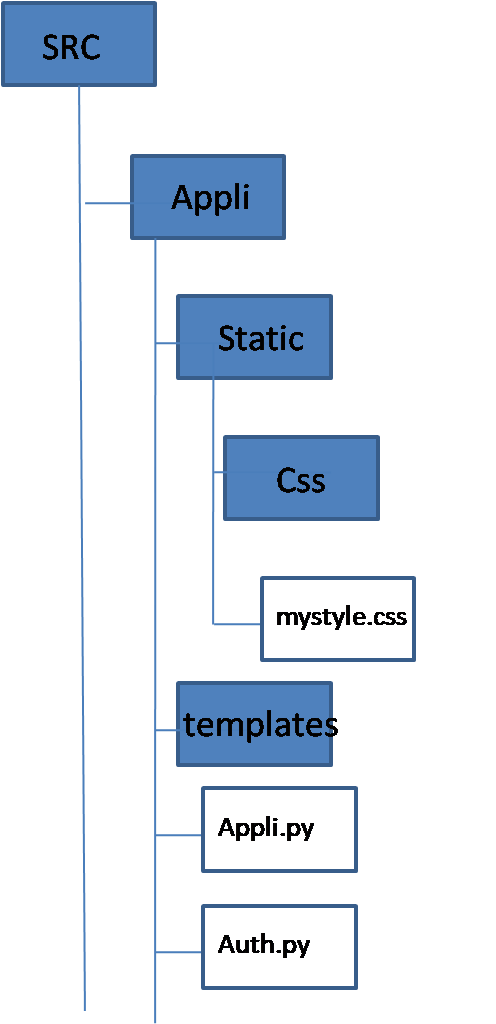
\includegraphics[width=5cm]{archifront.png}\\
         \textbf{Figure:}Architecture du Front-end
         \end{center}
 Les fichiers auth.py et appli.py qui instancient les formulaires contenant leur paramètre d'entrée ainsi que les templates HTML associés.
\subsubsection{Automatisation avec un script SH}
\textbf{launchapp.sh} permet de lancer l'application dans l'environnement virtuel de manière simplifiée afin de maximiser l'expérience de l'utilisateur.
 \subsection{Interface Graphique Générale}
 Il tient à préciser que le design graphique de notre application a pour inspiration le site officiel de l'Institut Mines-Télécom. La bar de navigation est commune à toutes les pages du sites et possèdent un bouton download qui à l'aide de URL obtenue par une fonction Javascript (request.url)
 \subsubsection{Bulma et Css}
 Pour le design de notre site Web, nous avons choisi le Flat Design plutôt que le Skeuomorphisme, qui permet de supprimer toutes les informations non-essentielles à l'utilisateur. Le choix de Bulma s'est donc imposé comme une évidence non seulement grâce à son utilisation pratique mais aussi grâce au design de ses assets, connus pour son flat design. Ainsi nous avons adapté à nos besoins les divers assets du sites ainsi pris pour inspiration en plus du color scheme et de la forme triangulaire. 
  \begin{center}
         
\includegraphics[width=3cm]{favicon.png}\\
         \textbf{Figure:}Icône de l'IMT modifiée pour signifier la notification 
         \end{center}
 De la même manière, nous avons implémenté un carrousel pour la page d'accueil à partir du fichier  mystyle.css dans lequel  sont implémentés un At-Rules keyframes modifiés ainsi qu'un At-Rules media adapté.

 \section{Partie Back-end de l'application}
 Il s'agit principalement des fonctions de création de base de données que l'on a présenté dans le chapitre précédent ainsi que l'installation de l'ensemble des dépendances de l'application. Nous avons également crée un script SH config.sh pour installer et configurer l'environnement du Back-end.
 \subsection{Architecture du Back-end}
 L'architecture est donc détaillée dans la figure suivante de manière simplifiée:
   \begin{center}
         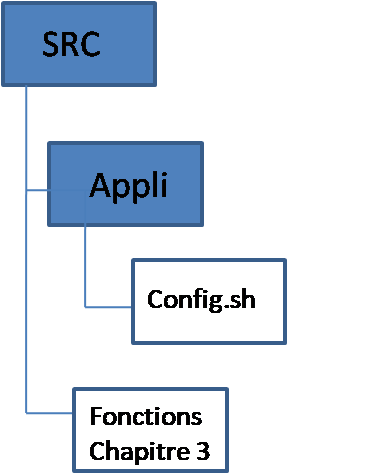
\includegraphics[width=5cm]{backendarch.png}\\
         \textbf{Figure:}Architecture du Back-end
         \end{center}\\
    Le Back-end utilise alors le principe de microservices, c'est à dire qu'ils utilisent plein de petits services différents plutôt qu'un code monolithique. Il y a plusieurs avantages à utiliser des microservices: mais celle qui ressort le plus c'est l'indépendance.En effet ces différents services sont testés et utilisés de façon indépendantes.
    
      \begin{center}
         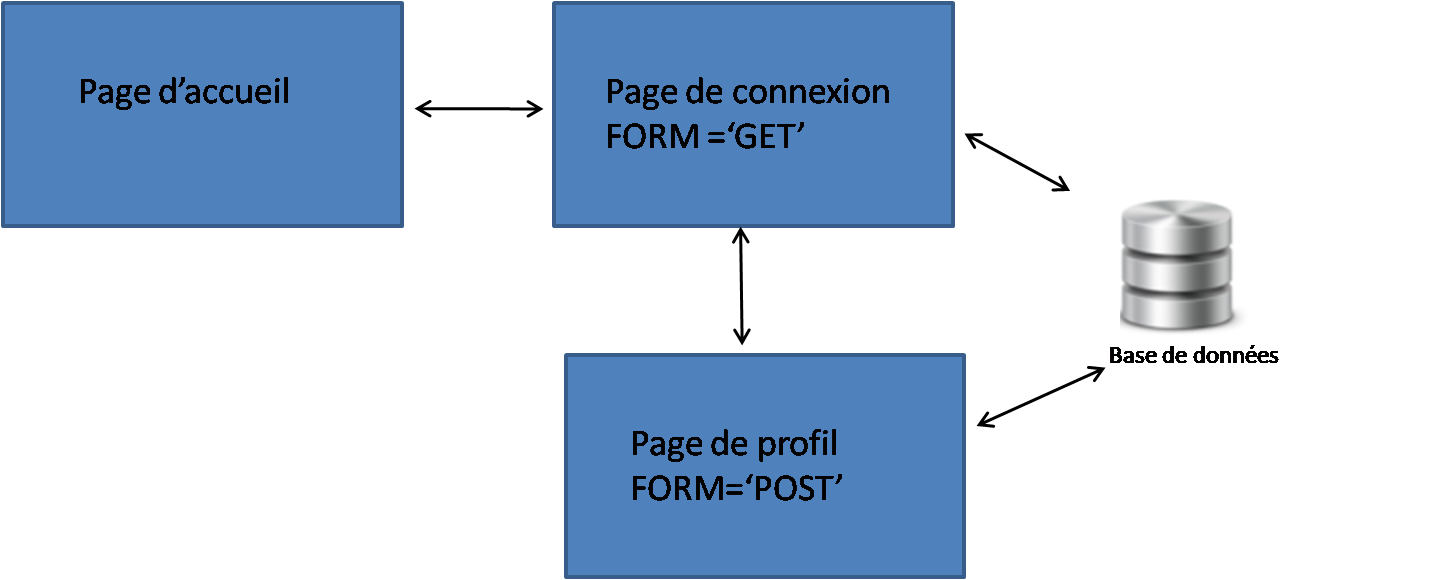
\includegraphics[width=15cm]{schsite.png}\\
         \textbf{Figure:}Architecture du site
         \end{center}\\

   \chapter{Gestion de Projet}
   \minitoc
      \section{Généralités}
      Ce projet se développe dans le cadre du module du P2II, il vise la mobilisation des connaissances acquises durant les différents modules de l'année scolaire, y compris la Gestion de Projet. \\
      
      Les algorithmes et leur étude développés lors de ce projet doivent répondre à l’énoncé fourni par Sébastien Da Silva et Gérald Oster. Tous les élèves participant au projet doivent travailler dans le déroulement de chacune de ses parties, autant comme développeurs que managers. Le projet s'est déroulé suivant le principe de la méthode Agile.\\


      \section{Outils de gestion de projet}
      \textit{Le bon outil pour le bon usage}.\\
      
      Pour bien gérer notre projet et pour respecter les consignes de l'énoncé, nous nous sommes appuyés sur plusieurs outils de gestion de projet:\\
      
      \begin{itemize}
         \item Charte de projet 
         \item Matrice SWOT
         \item Matrice RACI 
         \item Comptes-rendus rédigés lors de chaque réunion 
         \item Méthode Agile
      \end{itemize}
      
         \subsection{Charte de projet}
            
            \begin{itemize}
                \item {\textbf {Cadrage/Finalités et importance du projet}} \\
               \\
                
                \item {\textbf {Objectifs et résultats opérationnels}}\\
                

Tous les élèves participant au projet doivent maîtriser les différentes parties de l’application de tel sorte qu’ils soient capables de répondre à des questions sur ces dernières. Le projet se déroule par jalons définis à partir des sous-parties de l’énoncé.\\

Le projet vise à livrer une application, incluant une base de données et une méthode d’insertion de données depuis des fichiers excel et csv, qui sera notée.
Le projet cherche à répondre à la totalité des questions de son énoncé. On s’intéresse à la création d’une application qui permet l’utilisation et la modification d’une base de données créée à partir de fichiers fournis. Le développement et l’étude des fonctions algorithmiques, l’application résultante ainsi que la gestion du projet seront conçus par touts les participants et le compte-rendu final comportera un document rédigé sur Latex ainsi qu’une présentation orale accompagnée d’une démonstration. À l’issue du compte-rendu, le module sera soumis à une validation.  
\\


                
                \item {\textbf {Déroulement du projet/Organisation/ressources}}\\
                \begin{itemize}
                    \item Dans le déroulement de ce projet, les participants sont :\\
                    
                    LEDEUX Flavien\\
                    ROURA Guilhèm\\
                    ZHU Céline\\
                   
                    
                    Chacun des membres du groupe ont le même rôle en tant que développeur et manager.\\
                     \item Les moyens à disposition sont multiples :\\
                    - Logiciels de traitement de texte tel Latex\\
                    - Logiciels permettant travaille en équipe tel Gitlab\\
                    - Connaissances acquises lors de l'année scolaire 2020-2021 à TELECOM Nancy pour le développement et l’étude d’algorithmes\\
                    - Connaissances acquises lors du module de MOOC-GdP pour la gestion de projet\\
                    - Éventuelle aide des professeurs de TÉLÉCOM Nancy\\
                \end{itemize}
                \item {\textbf {Jalons : échéancier / événements importants}}\\
                
                 \begin{center}
         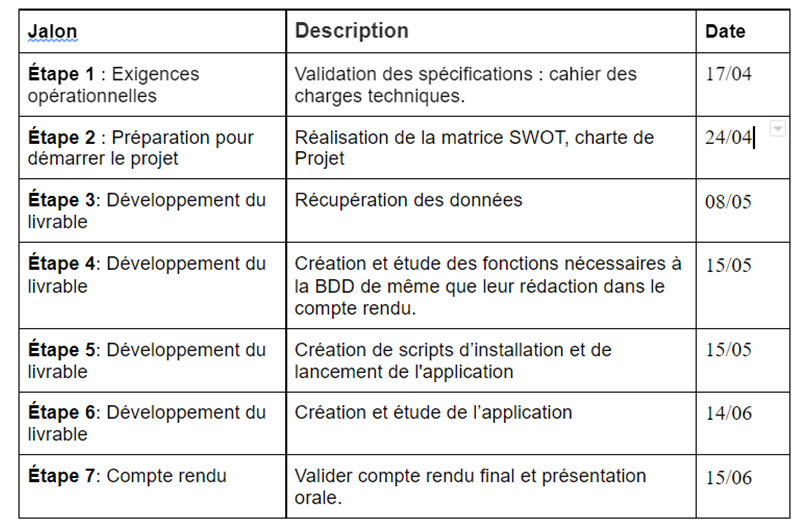
\includegraphics[width=15cm]{jalons.png}\\

         \end{center}

                \item {\textbf {Risques et opportunités}}\\
                Après analyse du déroulement du projet, on dégage:\\
                
                \qquad Plusieurs risques tels: \\
 - Un potentiel mauvais accès à internet\\
- Une absence de date butoir\\
- Le sujet n’est pas entièrement défini\\


	            \qquad Plusieurs opportunités telles:\\
-La possibilité de solliciter une personne extérieure au projet pour s'entraîner à la présentation orale\\

-La possibilité de demander de l'aide à un professeur en cas de blocage\\

-Accès à l’école et à son matériel\\
-Beaucoup de documentations en ligne\\

                 
                \end{itemize}   
                
            
                
            \subsection{Matrice SWOT}
    
                
                 \begin{center}
         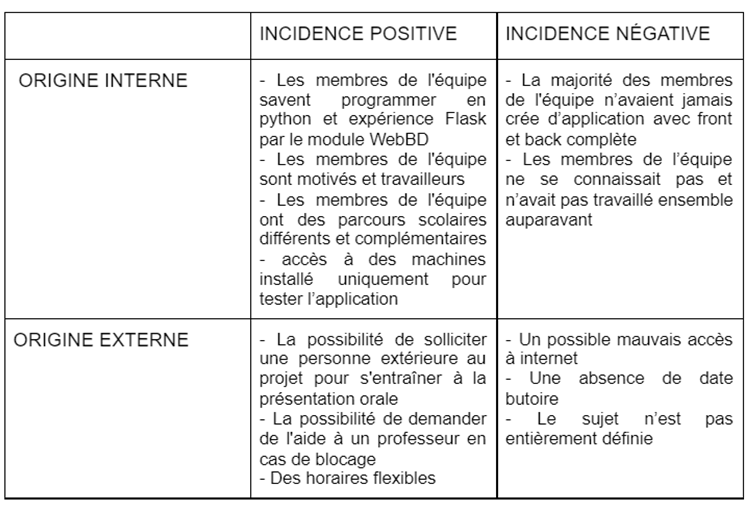
\includegraphics[width=15cm]{swot.png}\\

         \end{center}
    

         
        
        \subsection{Matrice RACI}
        
        Nous avons réalisé une matrice RACI dans le but de formaliser le rôle de chacun lors des différents lots de travail et avoir une idée claire de nos responsabilités. 
        
        La matrice RACI est illustrée par la figure ci-dessus.
         
       \subsection{Méthode Agile}
       En ingénierie informatique, la méthode Agile se base sur un cercle vertueux d'auto-discipline centrée sur la confiance en autrui et sur un feedback régulier. Nous avons décidé d'utiliser cette méthode plutôt que la méthode linéaire traditionnelle, car la méthode Agile permet des réponses très flexibles aux changements et aux imprévus. Étant donné la liberté donnée par le sujet, et le problème ouvert, nous avons donc décidé de ne pas s'embarquer dans une méthode trop rigide (Diagramme de Gantt), dans la situation où une grande modification du sujet ait lieux. Néanmoins, afin de se fixer une structure dans notre organisation, nous avons tout de même imposé des réunions dits de "vérification d'avancement". Ce sont des réunions non de travail, mais d'observation de l'avancement de l'équipe ainsi que de partage des difficultés rencontrées. Ces réunions ont donc été fixées à moins d'une heure et cette contrainte a été bien respectée à l'exception de deux réunions. Elle ont été plus focalisés sur la création de documents de gestion de projet.
        \subsection{Comptes-rendus}
        
        À l’issue de chaque réunion, un compte-rendu était rédigé pour résumer les propos traités, formaliser les décisions prises et la liste des responsabilités désignées à chaque membre de l’équipe pour la prochaine réunion. Sa rédaction était prise en charge par chacun d’entre nous de manière cyclique.

Chaque compte-rendu a été rédigé d'après le modèle donnée ci-dessous,la totalité des compte-rendus peuvent être retrouvés dans l'Annexe et sur le dépôt GitLab:
\title{P2II 1A - Compte-rendu n°1}
\begin{center}
        \begin{tabular}{|l|l|}
        \hline
   
\textbf{Motif de la réunion :}&\textbf{Lieu de la réunion :}\\

Réunion de démarrage du projet&Réunion en visioconférence sur Discord\\


        \hline
        \textbf{Présents :}&\\

Flavien LEDEUX&\textbf{Date :} 03/04/2021\\

Guilhèm ROURA&\\
Céline ZHU&\textbf{Heure :} 10h01\\

&\\
\textbf{Absent :}&\textbf{Durée :} 45 minutes\\

Personne&\\
&\\
\textbf{Rédaction du compte-rendu :}&\\

Céline ZHU&\\

        \hline
        \end{tabular}\\
        \end{center}
\minitoc


\section{Prendre connaissance du sujet}

Rapport sur la Gdp et la réflexion\\
    Objets à rendre:\\
    Base de données SQL standard + schéma\\
    Rapports formats html ( rédigé en fonction de quoi à demander à M Da silva ou M Oster)\\
Afficher les résultats des requêtes que ce soit en schéma ou par texte\\
L’état des fichiers final ou pas.\\
\section{Établir les outils de GdP}
Fichier Readme.md\\
Matrice RACI\\
Gantt \\
SWOT\\
\section{Établir le Cahier des charges}
Base de données SQL:\\
script Python rendant une base de données cohérente\\
Avec des informations\\
Trois étapes: Design, construction, tests boîte noire/blanche\\
	  - Application Python ( html):\\
			- Tous Flask\\
			- Définir tous les liens qui sont liés à notre application\\
			- Définir les conventions Html\\
			- Fiches de style\\
\section{Latex (?)}
Création du latex sur Overleaf et séparation en plusieurs fichiers Tex plus tard.\\
Programmation\\
 Flavien:  Python(flask) et Sqlite sont plus pratiques pour des amateurs. et on peut s’aider de la WebBD.\\

\section{ Planifier la semaine d'après }
	- Faire les scripts de la base de données pour les créer et le schéma.\\
		- Schéma: Flavien/Guilhèm\\
		- Scripts: Céline\\
		- Tests: Flavien/Céline\\
	-Commencer à réaliser les classes représentant les différentes éléments à ajouter dans la BDD.\\
	- Documenter vos actions en latex.\\
Prochaine réunion:\\
Samedi à 10h01 10/04/21:\\
	odj: \\
- Avancement du projet\\
	- Construction de la matrice RACI\\
	- Faire le Gantt\\
	- Dire les endroits qui nous ont posés problèmes\\


      \section{Organigramme projet}
      
      Selon leur localisation dans l'organigramme, il existe 3 types de projets:
      
      \begin{itemize}
          \item Au sein d'un même service: c'est un \textit{projet local}.
          \item Impliquant plusieurs services différents: des \textit{projets transversaux}.
          \item \textit{projets sortis}: de taille importante et font appel à des intervenants détachés spécialement.
      \end{itemize}
      
      Notre projet est clairement un projet transversal au sein d'une structure fonctionnelle.
      
      En effet, la structure fonctionnelle est une structure où il n'y a pas de chef de projet, ce qui encourage l'initiative, favorise l'adaptation aux évolutions de l'environnement et facilite la circulation des informations. De plus, la division du travail se fait par fonctions ce qui favorise l'efficacité du travail.
      
      Cette structure a permis à chacun d'entre nous de décider quelles tâches leur a été confiées:
      
      \begin{itemize}
          \item \textbf{Flavien Ledeux}
          \begin{itemize}[label=$\bullet$]
              \item réalisation des script de création de la base de données (BDDCreation.py)
              \item réalisation du script d'upload des données vers la base de données depuis un répertoire (ImportRepository.py)
              \item réalisation des script d'installation automatique installer (Windows et Linux)
              \item mise en place du polymorphisme sur les fonctions de lecture de fichier et création d'une fonction l'utilisant pour retourner les informations du fichier
              
              \item création des tables notes, voeux\_ecole et ranginfo ainsi que les tables qui dépendent de ces dernières
              \item mise a jour et correction du schéma de la base de données
              
              \item Réalisation des fonctions Add sous leur forme initial
              \item réalisation des fonctions qui insèrent des informations vers la base de données sauf pour les fichiers inscription et listeEtablissement (\ref{tab:TableKeyChar} page \pageref{tab:TableKeyChar})
          \end{itemize}
          
          \item \textbf{Guilhèm Roura}
          \begin{itemize}[label=$\bullet$] 
              \item Réalisation d'une partie du schéma de la BDD, notamment la table candidat.
              \item Réalisation de l'insertion des données provenant du fichier Inscription.
              \item Fonction d'insertion dans la BDD (\textit{InsertData} et \textit{InsertOrUpdateData})
              \item Modification des fonctions Add pour supprimer le redondance du code d'insertion des tables, en utilisant les 2 fonctions ci-dessus
              \item Fonction de statistiques et de test.
              \item Relecture et corrections diverses dans les différentes fonctions
              
          \end{itemize}    
          \item \textbf{Céline Zhu}: 
                \begin{itemize}[label=$\bullet$] 
              \item Réalisation d'une partie du schéma de la BDD, notamment la création des tables adjacentes à la table candidats et de leurs jointures
              \item réalisation des scripts de lecture des fichiers Excel et CSV
              \item réalisation de la fonction d'upload des données pour listeEtablissement
              \item réalisation de l'application Flask
              \item réalisation des fichier .sh pour automatiser Flask et automatiser la création de l'environnement virtuel nécessaire
          \end{itemize}
      \end{itemize}
      
      
      
\chapter{Conclusion}

Tout d'abord, nous avons pris du temps à démarrer. Bien que nous nous soyons rapidement mis d'accord sur les technologies à utiliser, nous avons pris beaucoup de temps à concevoir la base de données.\\

Pour 2 raisons: tous d'abords, il y a plusieurs fichier, et en particulier "Inscription", qui contiennent beaucoup de colonnes.\\

Il fallait donc être rigoureux pour ne rien oublier, mais tout en veillant à n'avoir que des tables et des attributs pertinents. En effet,
il fallait respecter la contrainte de normalisation de la table, et éviter aux maximum les redondances.\\

De plus, il y a globalement de nombreux fichiers, et de nombreuses données dans chacun d'eux. Tout était plus ou moins liés, ce qui augmentait la complexité.
De plus, cette intrication entre les fichiers et les tables rendaient plus difficile de travailler à plusieurs simultanément sur le schéma de la base de données.\\


Pour l'application, nous avons bien réussi à travailler ensemble et à avoir un code aussi propre que possible. Cela est passé notamment en ayant de nombreux fichiers différents pour séparer les différents domaines de l'application. Nous avons de plus veillé à créer des fonctions simples et assez courtes ne faisant qu'une chose à la fois. Nous les avons documentées, afin de savoir ce qu'elle font, prennent en argument et renvoie. Cela à permis de facilement travailler à plusieurs sur la même chose en parallèle, et de pouvoir comprendre et corriger le code des autres avec aisance.\\


Pour la gestion de projet, les différents documents fait au début du projet, et complété éventuellement par la suite, ont permis de savoir quoi faire. 
Nous avons ainsi évité de nous disperser sur des idées ou des conceptions différentes.\\

De plus, nous étions tous les 3 à l'aise avec la méthodologies que nous avons suivi, consistant à travailler de notre côté.
Nous mettions en commun notre avancé et nos problèmes lors de réunion hebdomadaire de généralement 30 à 45min. Elles ont rarement dépassé 1h, lors de réflexions et travails en commun, notamment pour des documents de gestion de projet ou modification de la base de données.




\section{Conclusion personnelle }
\subsection{LEDEUX Flavien}
J'ai trouvé ce projet intéressant car les informations vis à vis du projet venaient petit à petit et que le sujet restait vague mais laissant la possibilité d'être précisé à l'aide de questions, ce qui est quelque chose qui ressemble à un exemple concret de projet que l'on risque de rencontrer dans le futur.

D'autre part, ce projet m'a permit de me familiariser avec un langage qui m'était presque inconnu : le langage des fichiers batch ainsi que de revoir les scripts bash que j'avais vue au tout début de ma formation d'IUT.

De plus le projet m'a permis de travailler avec des personnes qui m'étaient inconnues confrontant ainsi mes méthodes de travailles à celles des autres forçant ainsi une adaptation enrichissante dans le but de garder le meilleur de chacun.

Je trouve cependant que notre projet n'as malheureusement pas atteint toutes les attentes que j'avais vis à vis de ce dernier. Cela est pour de multiples raisons telles que le manque de temps pour approfondir certaines thématiques, la présence des partiels lors de la fin de projet limitant le temps disponible a consacrer a ce dernier et un investissement plus important possible vis à vis du projet.   

Si je devais refaire le projet de zéro, j'essaierais de mieux gérer la l'utilisation de notre temps en nous planifiant mieux et en séparant mieux les différentes tâches. 
De plus, j'essaierais aussi de nous faire travailler avec une cadence plus importante sur le début du projet.

D'autre part, la chose que j'essaierais le plus d'appliquer à d'autres projets est notre méthode rigoureuse de planification et d'exécution des réunions qui nous a permis d'éviter de rester bloquer trop longtemps.
D'autre part, le contenu des réunions était toujours pertinent et le travail était au rendez-vous lors de ces dernières ce qui ce reflète dans des temps de réunion ne dépassant qu'occasionnellement une heure.

Enfin, ce projet m'as forcé a prendre du recul vis a vis de ma méthode de travailler car j'ai du développer un rôle plus en retrait vis à vis de la création de la base de données pour pouvoir laisser mes collègues gagner de l'expérience avec cette notion au lieu de me concentrer la faire a ma façon au détriment de mes collègues.

Pour conclure, j'ai trouvé ce projet enrichissant bien qu'il laisse un arrière goût amer en quand on réfléchit à ce qui aurait pue être amélioré où rajouter.


\subsection{ROURA Guilhèm} Ce projet fut mon premier projet complet, allant de la conception à la réalisation.
J'ai d'abord pu m'entraîner et m'améliorer à la conception d'une base de données, chose que je ne maîtrisais pas forcément au départ.
J'ai pu bien prendre conscience et mettre e pratique des concepts tel que la normalisation d'une base de données, ou encore la manière d'éviter la redondance par des tables auxiliaires.

Pour ce qui est de la programmation, cela ma permis de faire mon premier projet complet en python.
Je me sentais déjà assez à l'aise avec, mais je n'avais jamais fait de projet de cette ampleur.

De manière général, j'ai pu me rendre compte de la difficulté et la complexité d'entière concevoir une application qui soit solution à un problème précis.
La liberté de conception permet de se sentir réellement impliqué et de faire des choix en fonction de ses préférences et de ce qu'on juge le plus pertinent.

Cette liberté est cependant à double tranchant: Il faut savoir se fixer des limites pour ne pas rester bloqué sur la phase de conception, tout en étant aussi rigoureux que possible. 
Tous les mauvais choix auront des répercussions par la suite, ils peuvent obliger à s'adapter lors de la phase de réalisation, par exemple en raison du langage et des technologies utilisées.
Mais la conception même peut être à revoir, par exemple pour le schéma de la base de données, si cette dernière ne répond finalement pas à toutes les problématiques posés.
On peut aussi la revoir si une solution bien meilleur est trouvée par la suite.


Enfin, ce projet fut le premier que je fais avec des personnes que je ne connais pas, et ayant des parcours différents.
Ces différences m'ont cependant semblé être plus des forces que des faiblesses, puisque chacun à ses propres points forts et connaissance à apporter.
Le fait de devoir adapter sa méthode de travail m'a semblé valoir le coup, puisqu'on peut tenter de garder le meilleur de chacun en terme de méthode.
De plus, chacun s'est investi et s'est senti responsable du projet, dans l'échec comme dans la réussite, ce qui constitue une bonne synergie, et nous a permit de rester motivé. 


Pour finir, mon ressenti sur le projet est que le temps pris au début pour concevoir la base de données et commencer les scripts python fut trop important.
Cela à laissé moins de temps pour avoir un résultat satisfaisant.
Cependant, la grande complexité des données à analyser a obligé à prendre du temps pour bien tout comprendre et tout concevoir correctement.

\subsection{ZHU Céline}

La différence entre théorie et pratique m’a parfois surprise durant la réalisation de ce projet que ce soit en gestion de projet ou en informatique.\\ L'approfondissement du Flask par exemple a été une expérience enrichissante allant au delà des cours fournis et allant dans le domaine de la recherche personnelle. C'était toujours très gratifiant de faire réussir à coder un nouveau bout du site et d'interagir très rapidement avec.\\

La réalisation de mon premier projet complet ne vient cependant pas sans défaut. En effet, nous avons eu la chance d'avoir un sujet qui nous laissez beaucoup de liberté et parfois ne maîtrisant pas bien mes limites, je me lançait dans des projets trop ambitieux pour mon niveau: par exemple le carousel qui a été très chronophage pour un rendu finalement qui n'était peut-être pas tellement intéressant.\\

C'est aussi mon premier projet en méthode Agile avec des gens que je ne connaissais pas. Heureusement, nous avions eu des complémentaires grâce à des parcours scolaires très différents nous permettant ainsi sur beaucoup de niveau de nous combler nos lacunes.\\

Qu’est-ce qu’on pourrait améliorer ? Beaucoup de choses, mais je citerai trois
points clés : un démarrage en gestion de projet plus rapide, une sauvegarde plus automatique des fonctions codées et enfin être moins optimiste quant aux dates buttoirs. Ce premier projet d’informatique m’a permis de vérifier la bonne acquisitions des compétences acquise durant cette première année à TELECOM Nancy.En conclusion, ce fut une expérience enrichissante qui s’est très bien passée dû à la synergie de travail du groupe.
\nocite{*} 
\printbibliography

\chapter{Annexe}

\section{Schéma de la base de données A}
\label{pdf:schemaBDD}
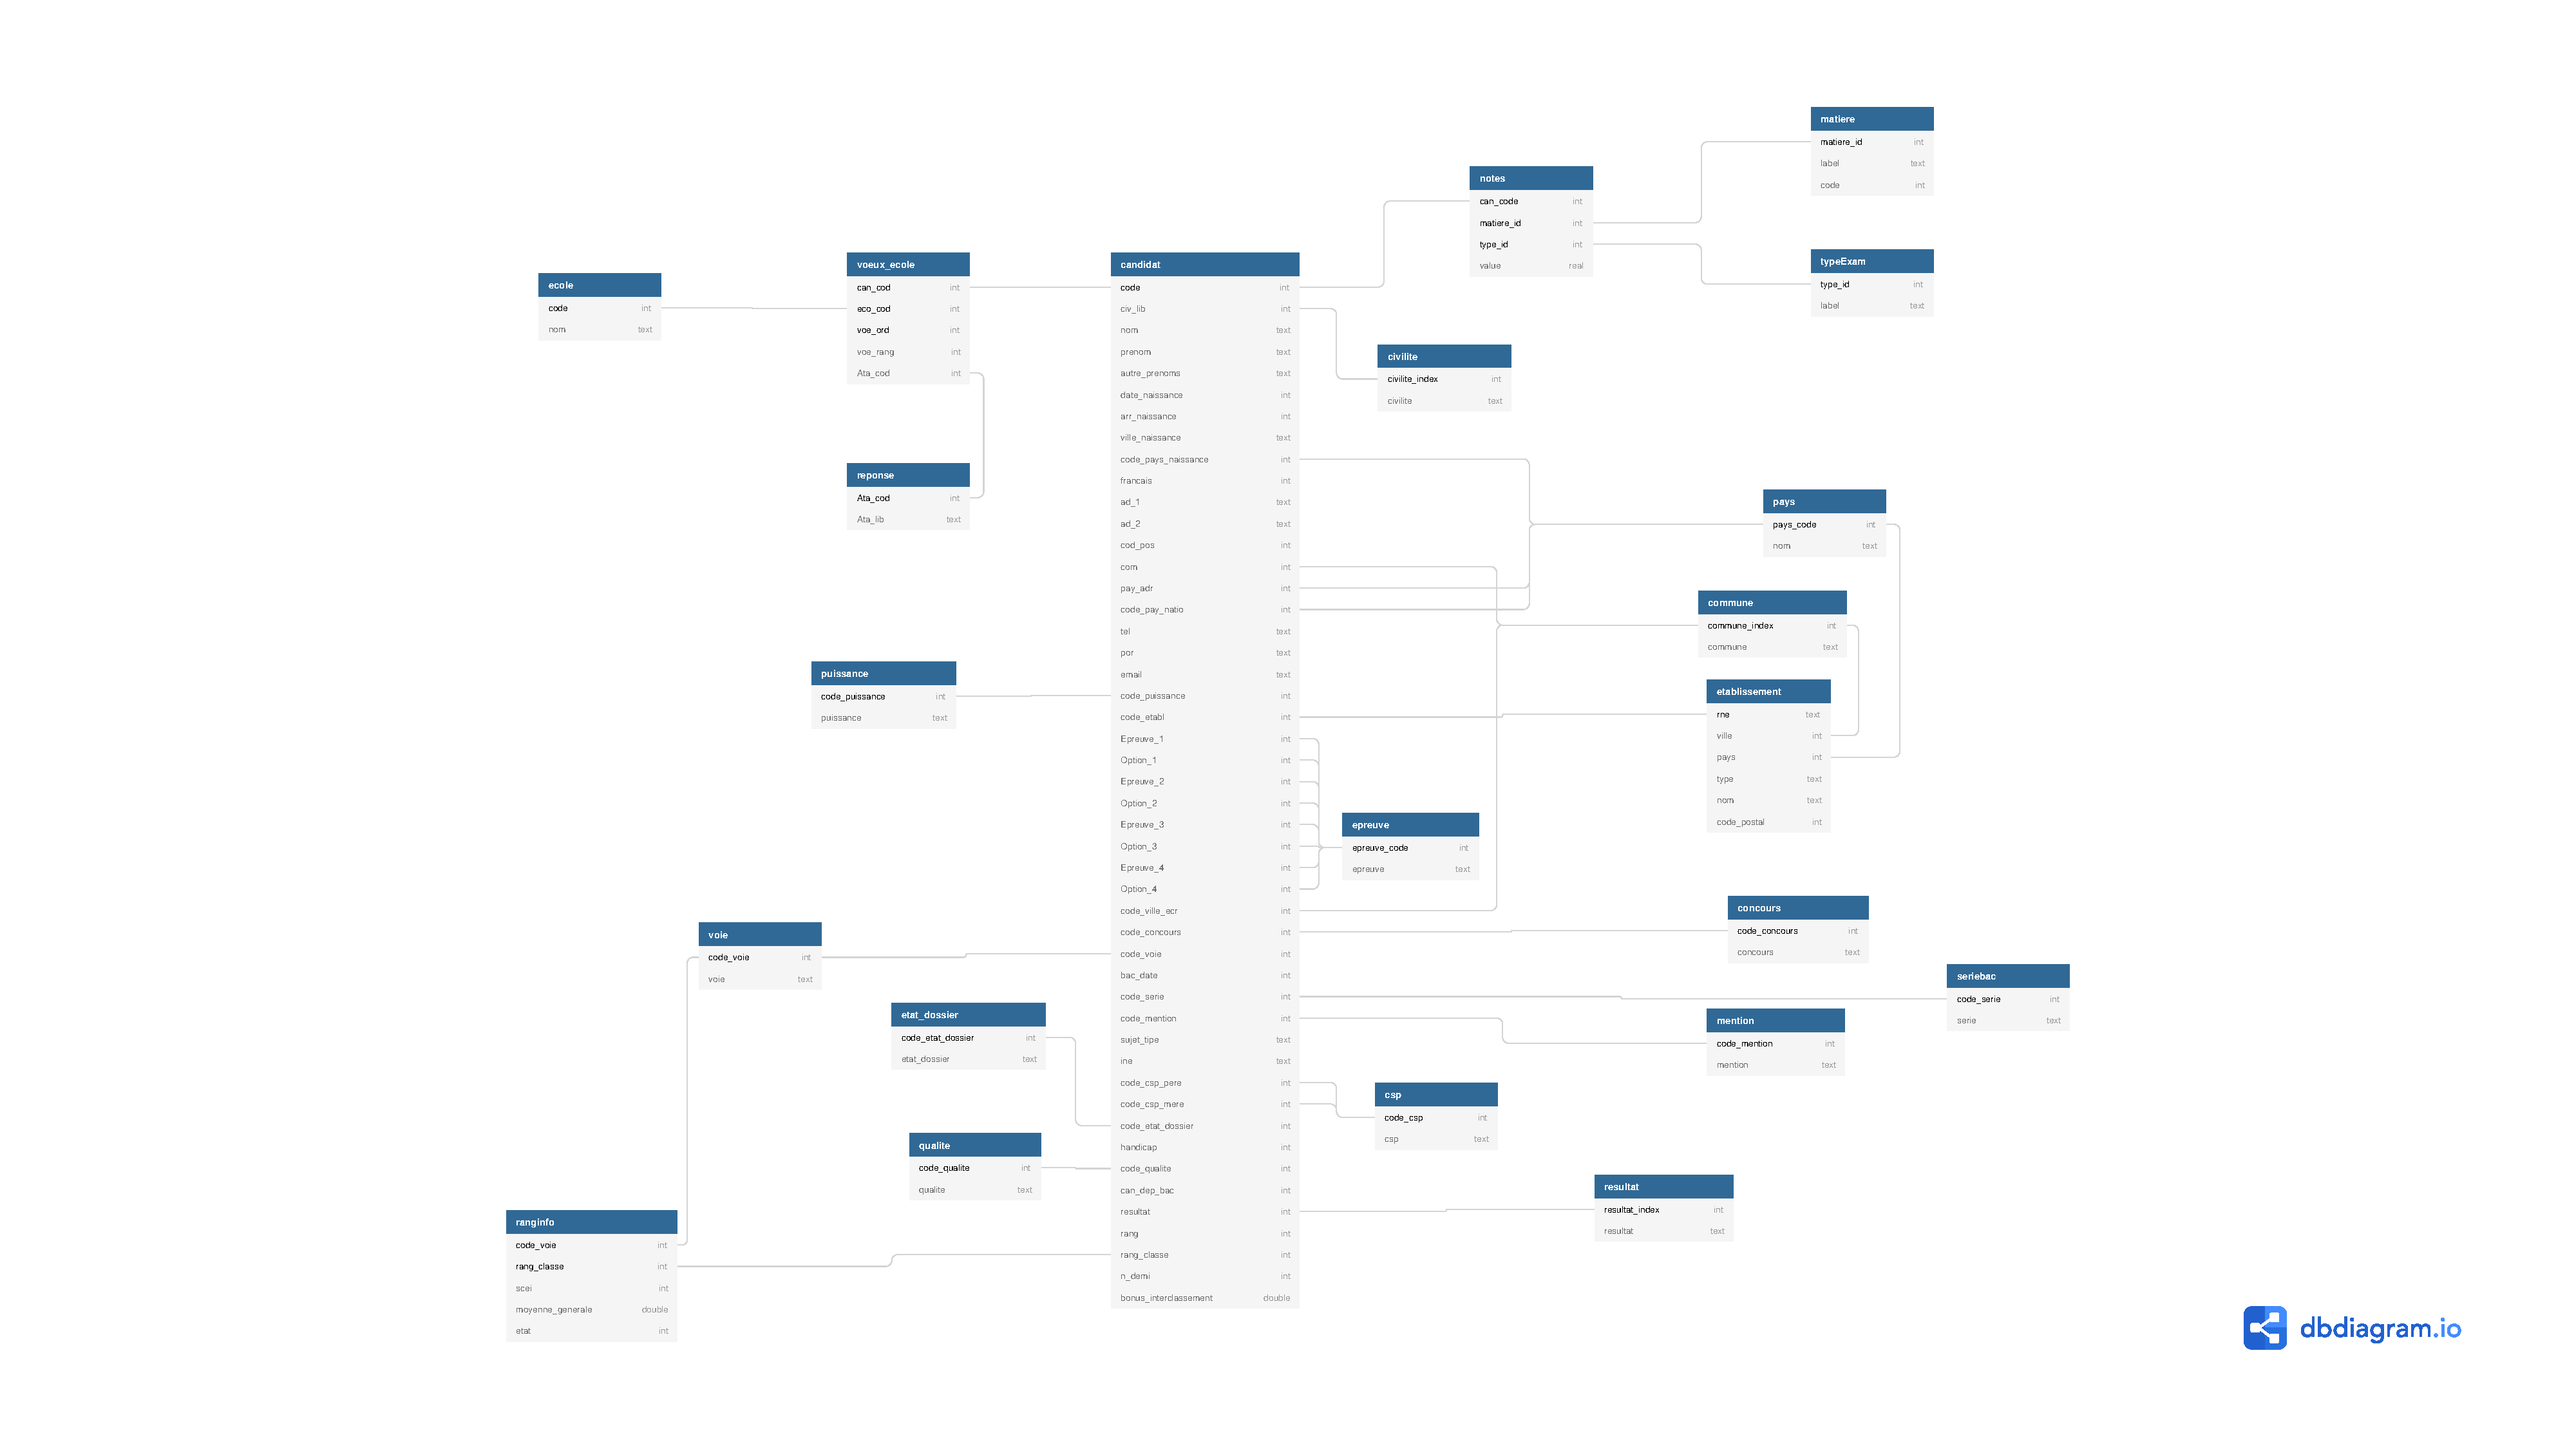
\includepdf[pages=-]{pdf/Schema.pdf}
\label{pdf:CR1}
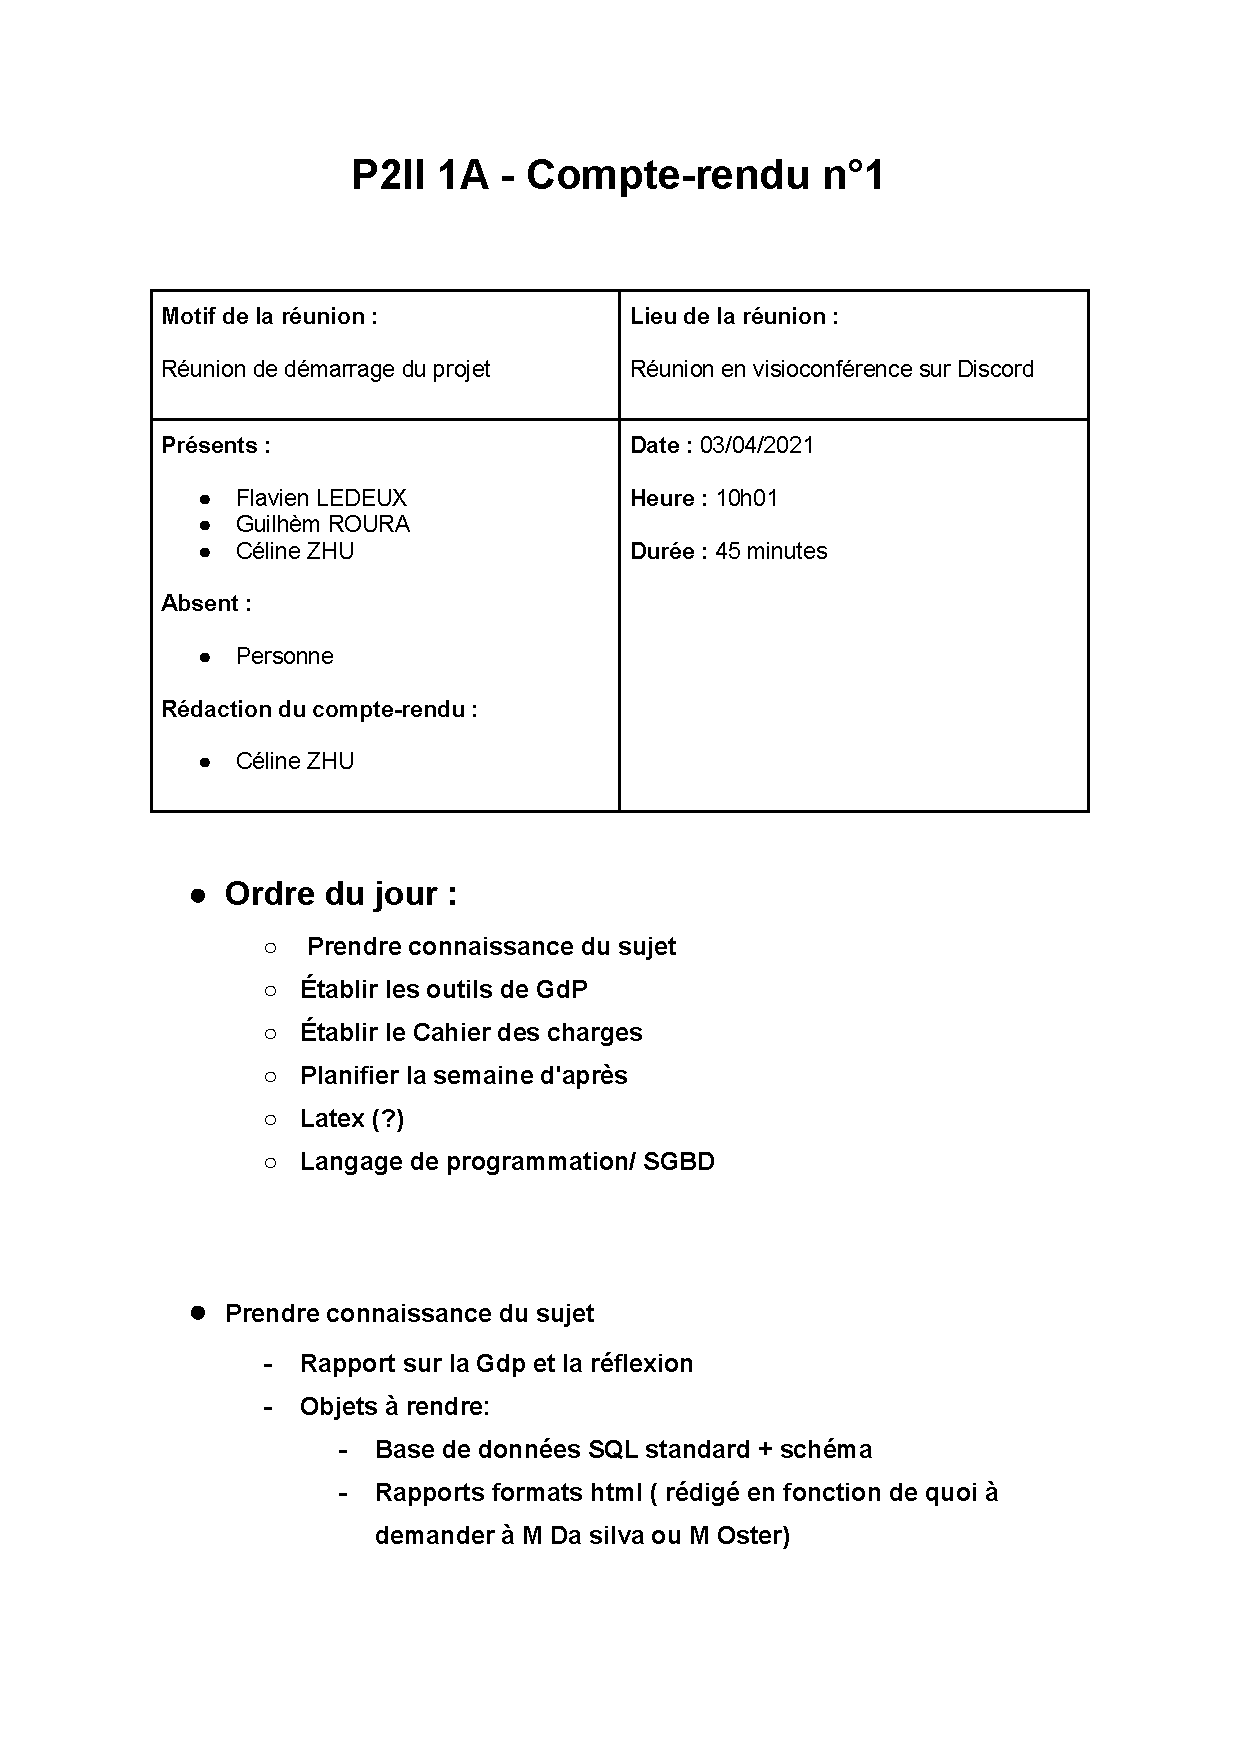
\includepdf[pages=-]{pdf/P2II_1A-Compte-rendu_n1.pdf}
\label{pdf:CR2}
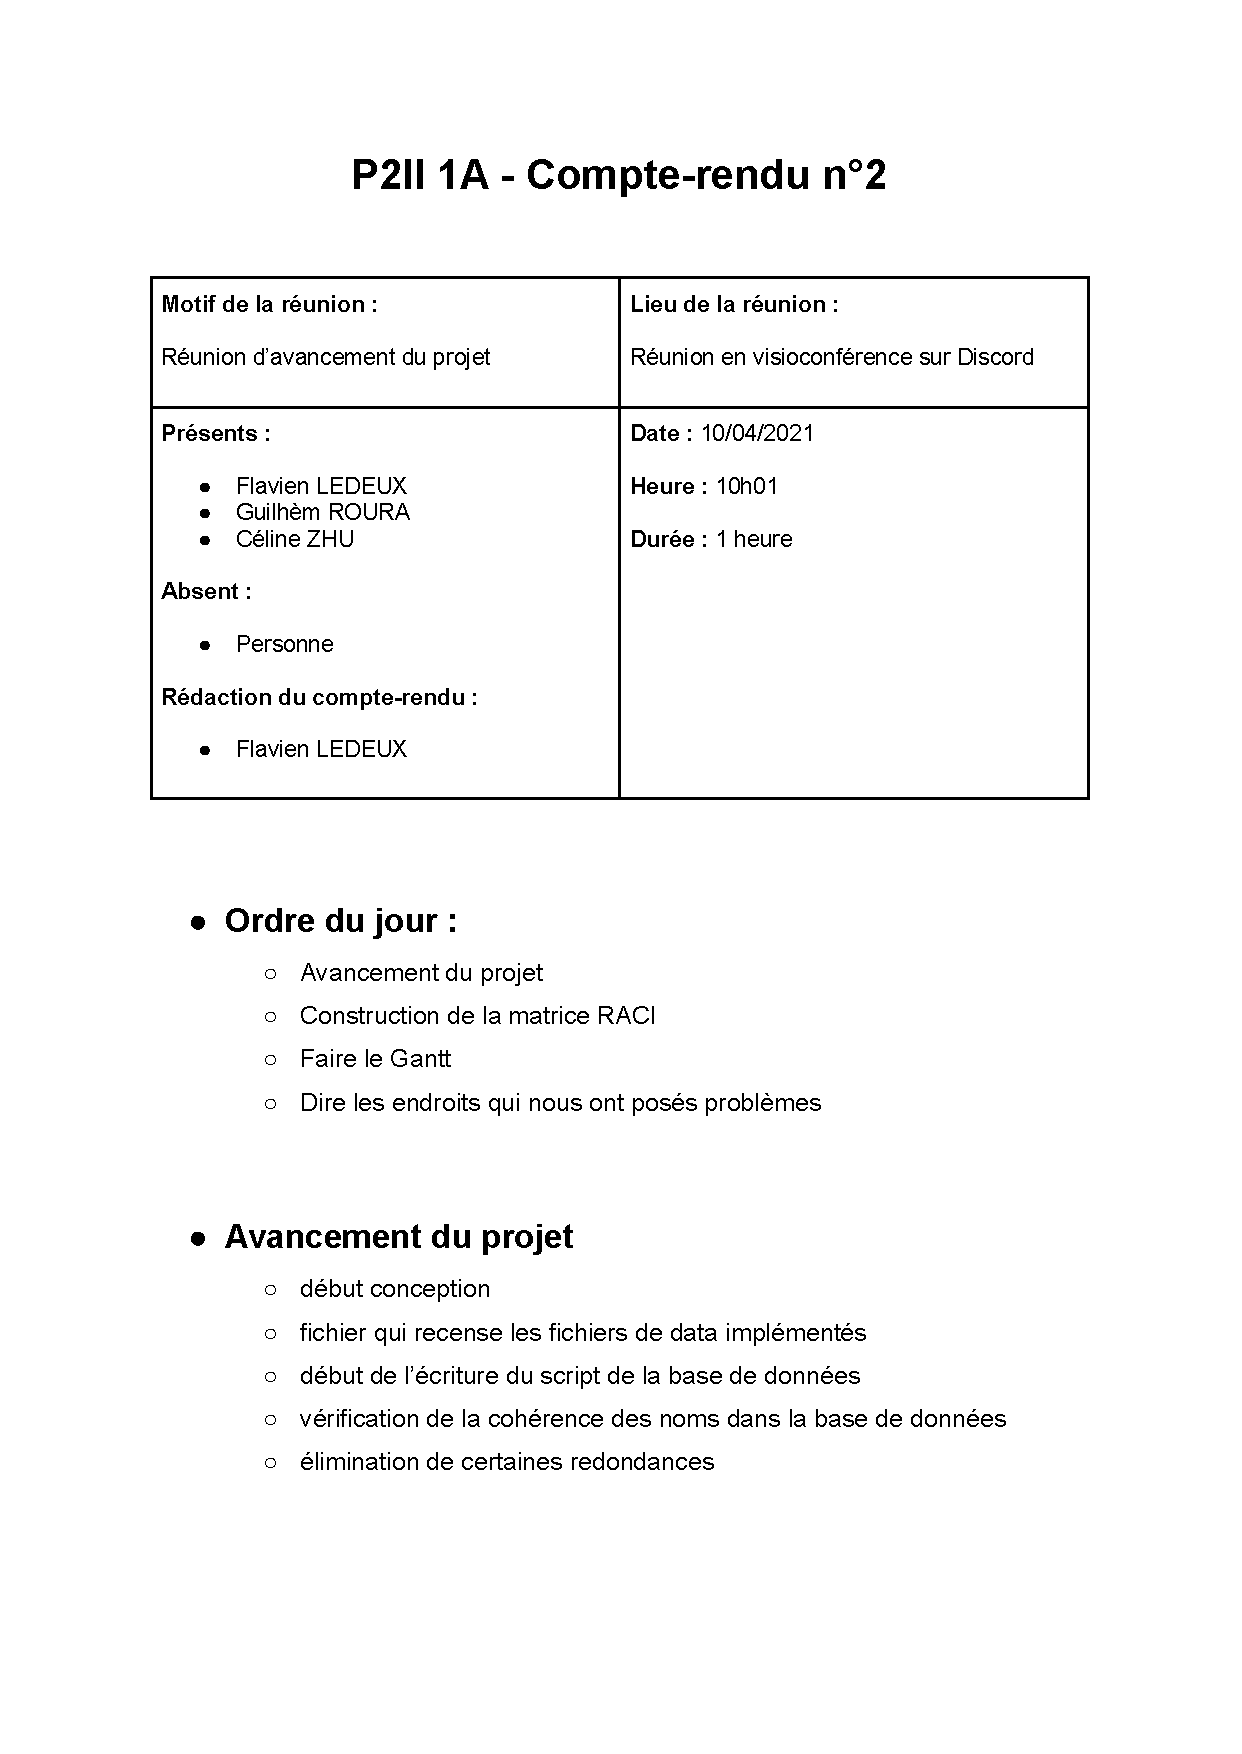
\includepdf[pages=-]{pdf/P2II_1A-Compte-rendu_n2.pdf}
\label{pdf:CR3}
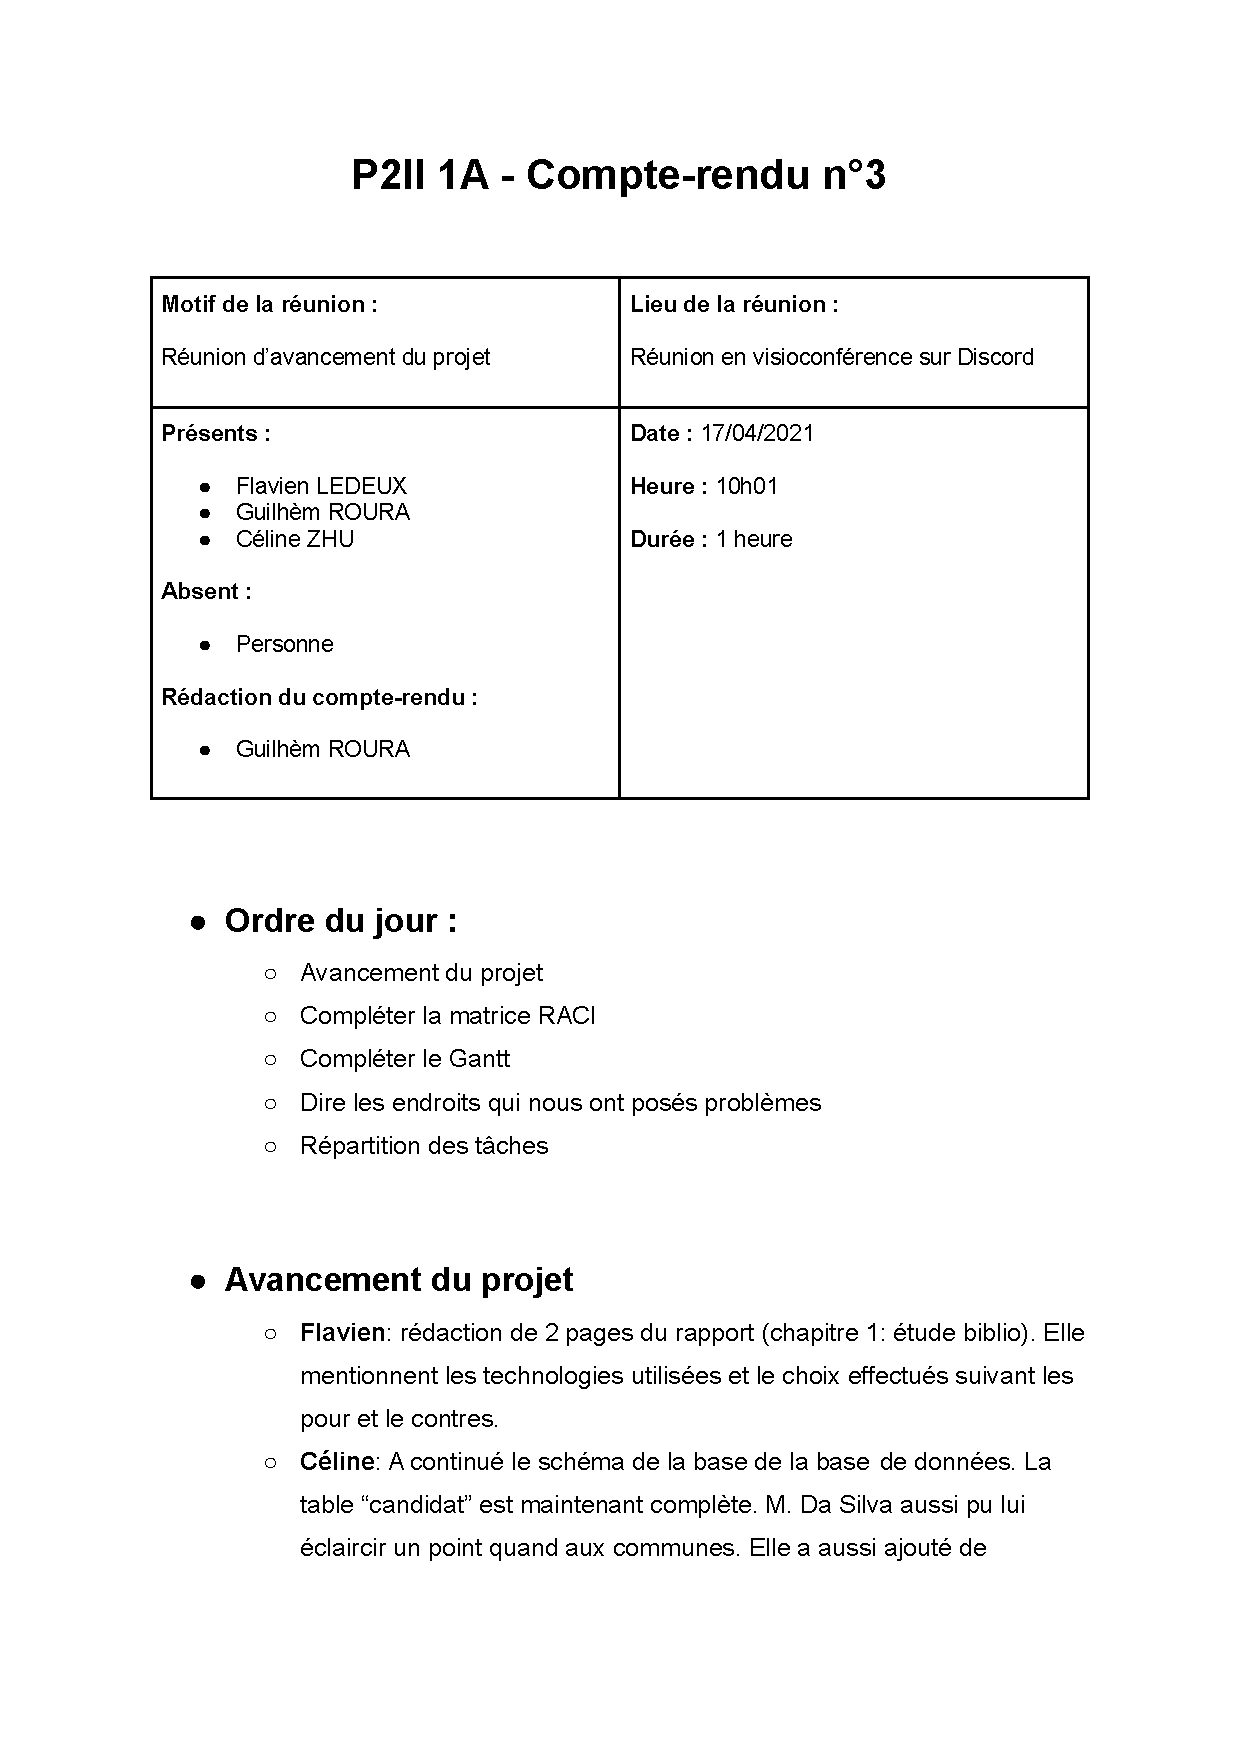
\includepdf[pages=-]{pdf/P2II_1A-Compte-rendu_n3.pdf}
\label{pdf:CR4}
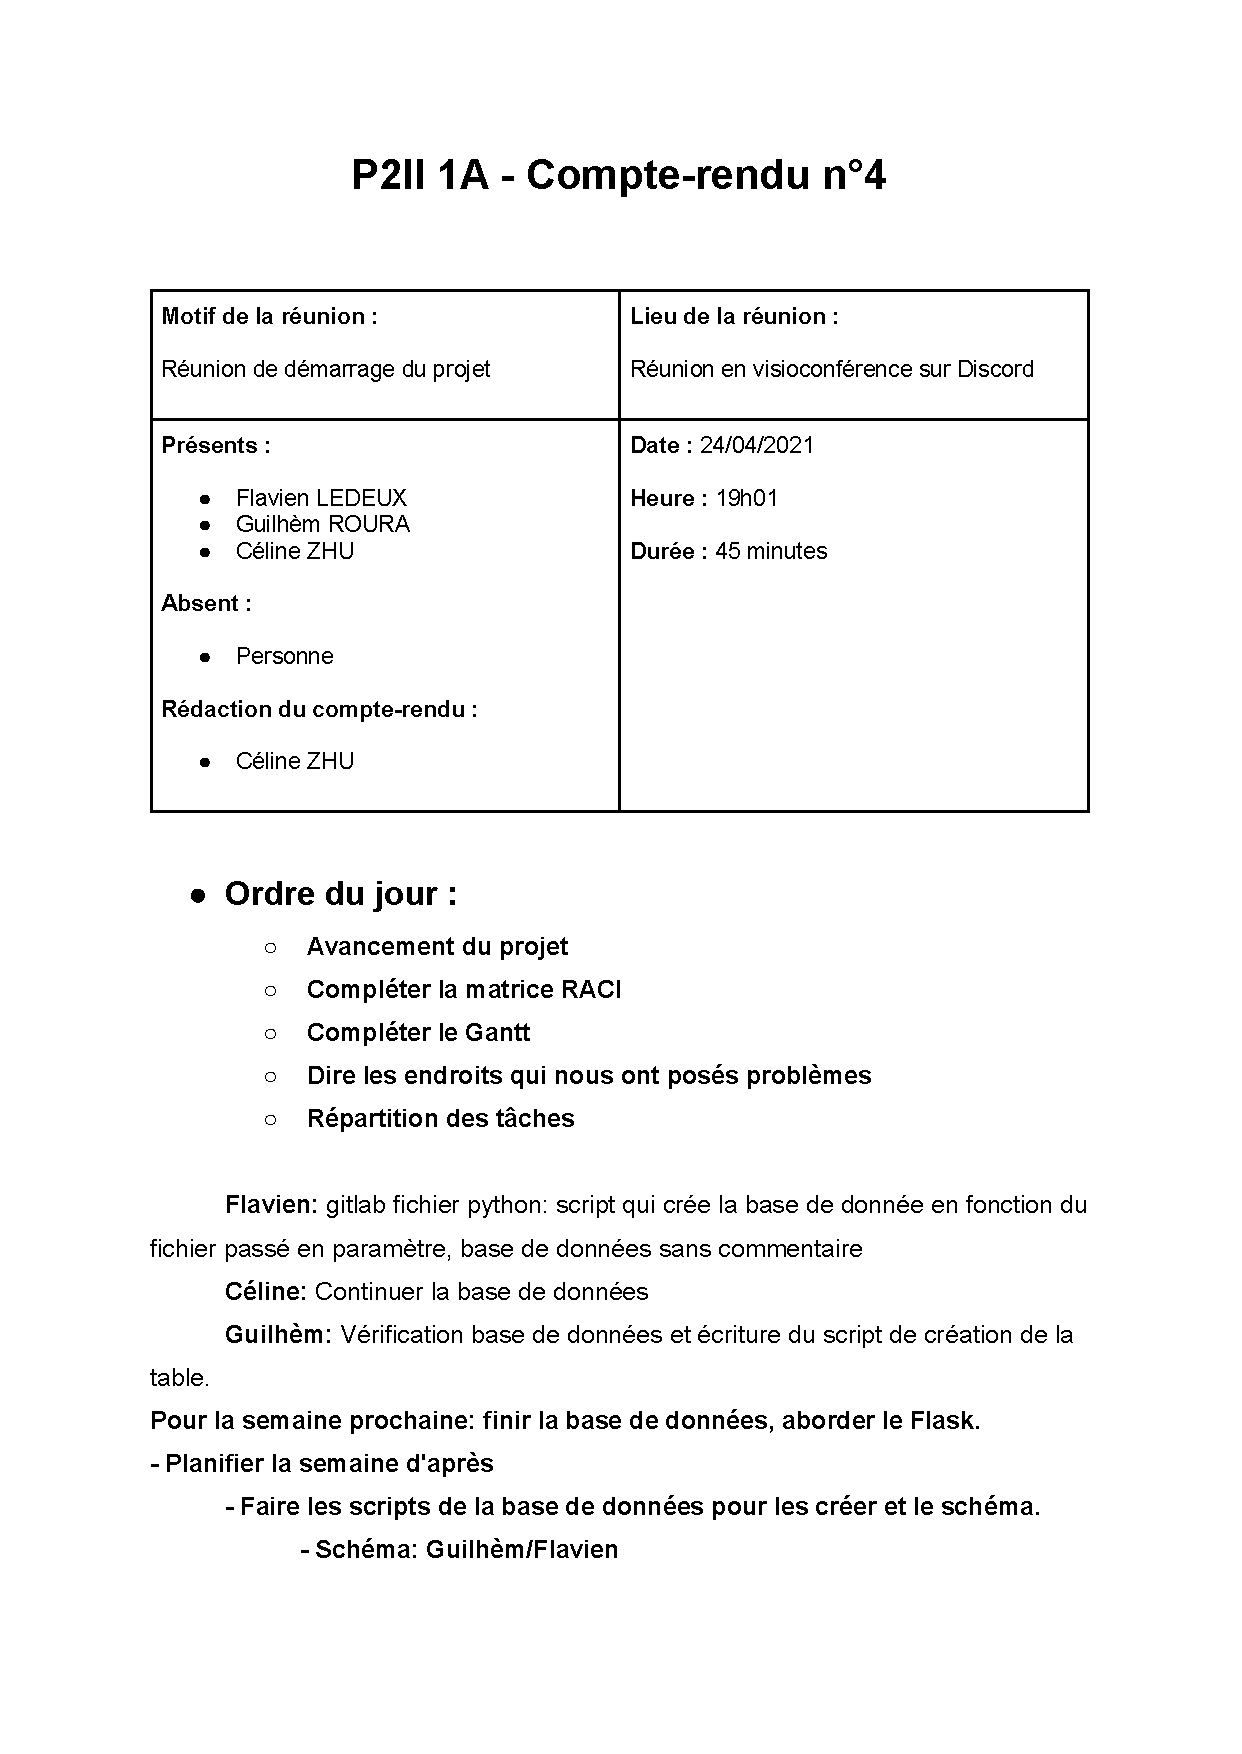
\includepdf[pages=-]{pdf/P2II_1A-Compte-rendu_n4.pdf}
\label{pdf:CR5}
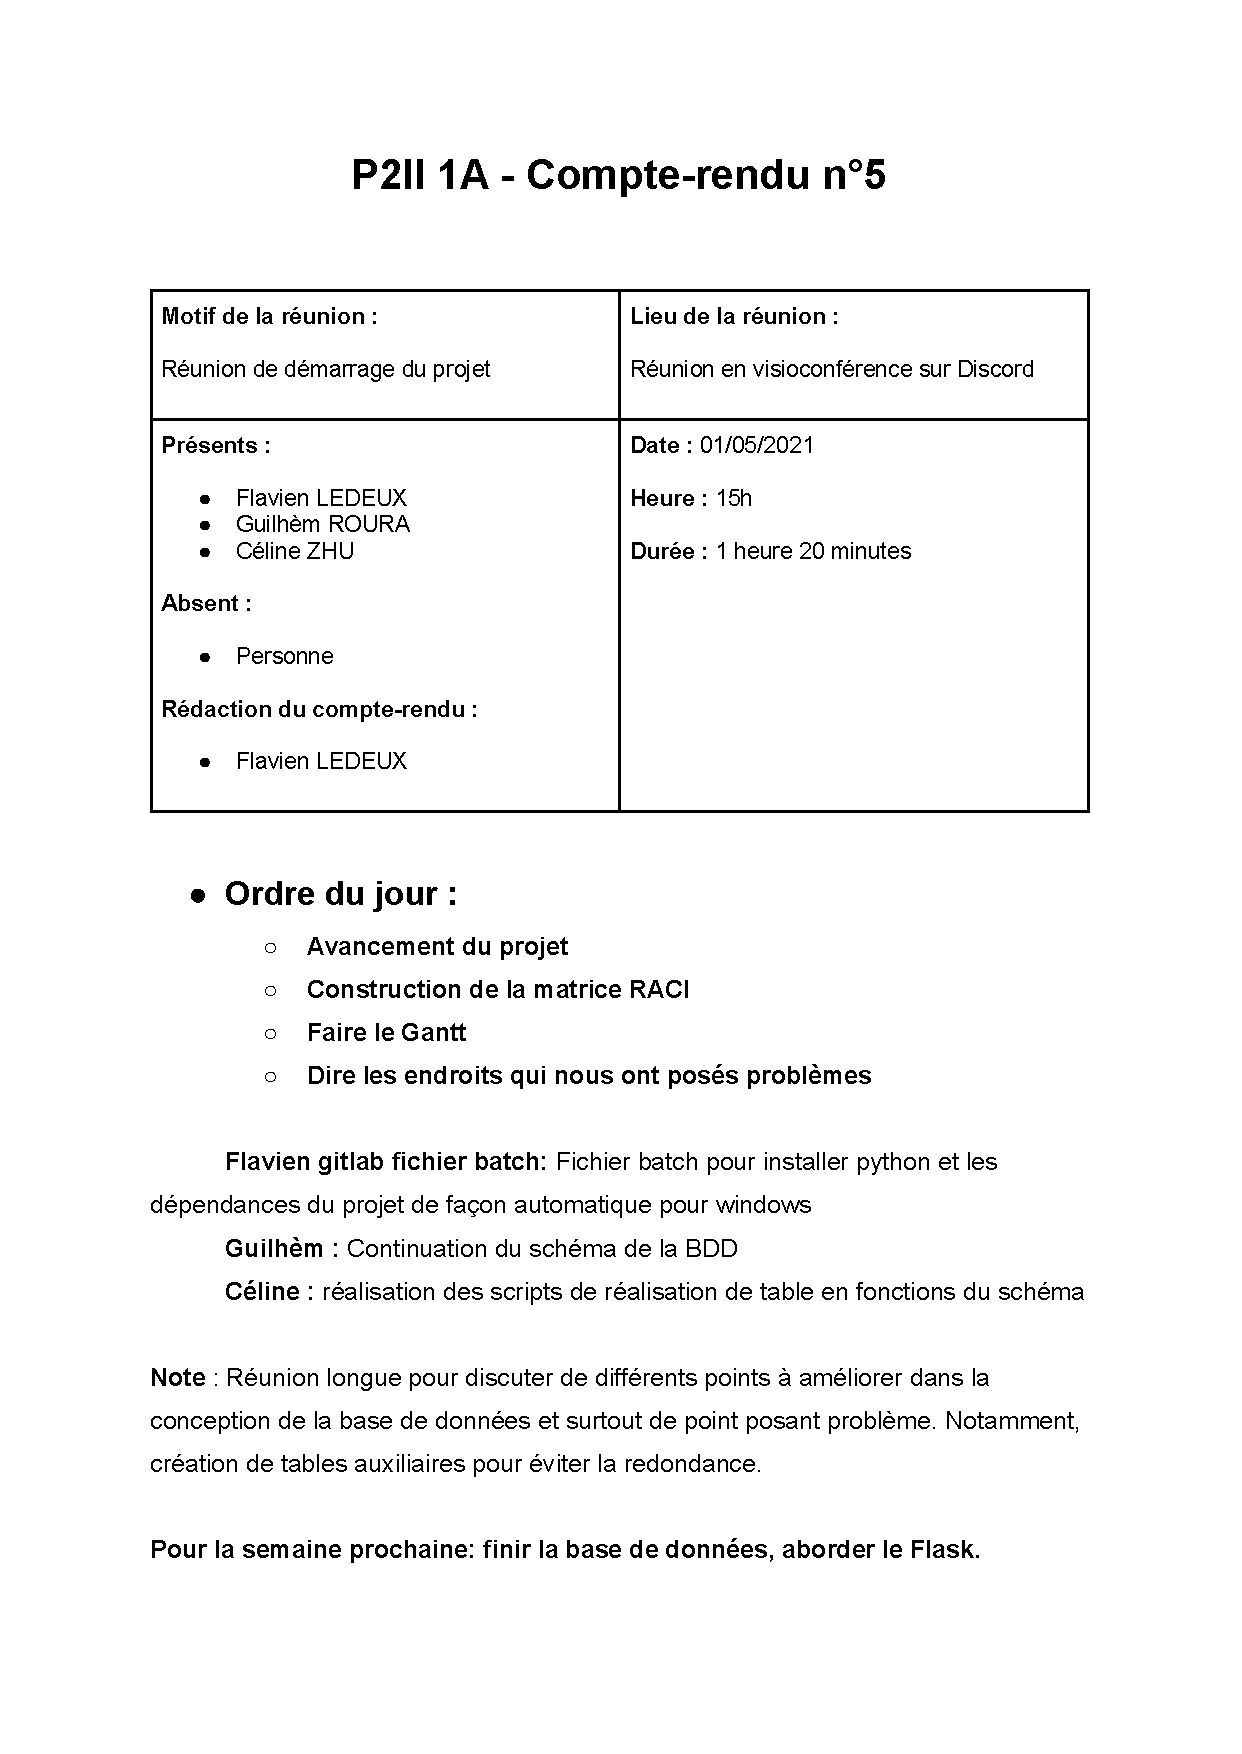
\includepdf[pages=-]{pdf/P2II_1A-Compte-rendu_n5.pdf}
\label{pdf:CR6}
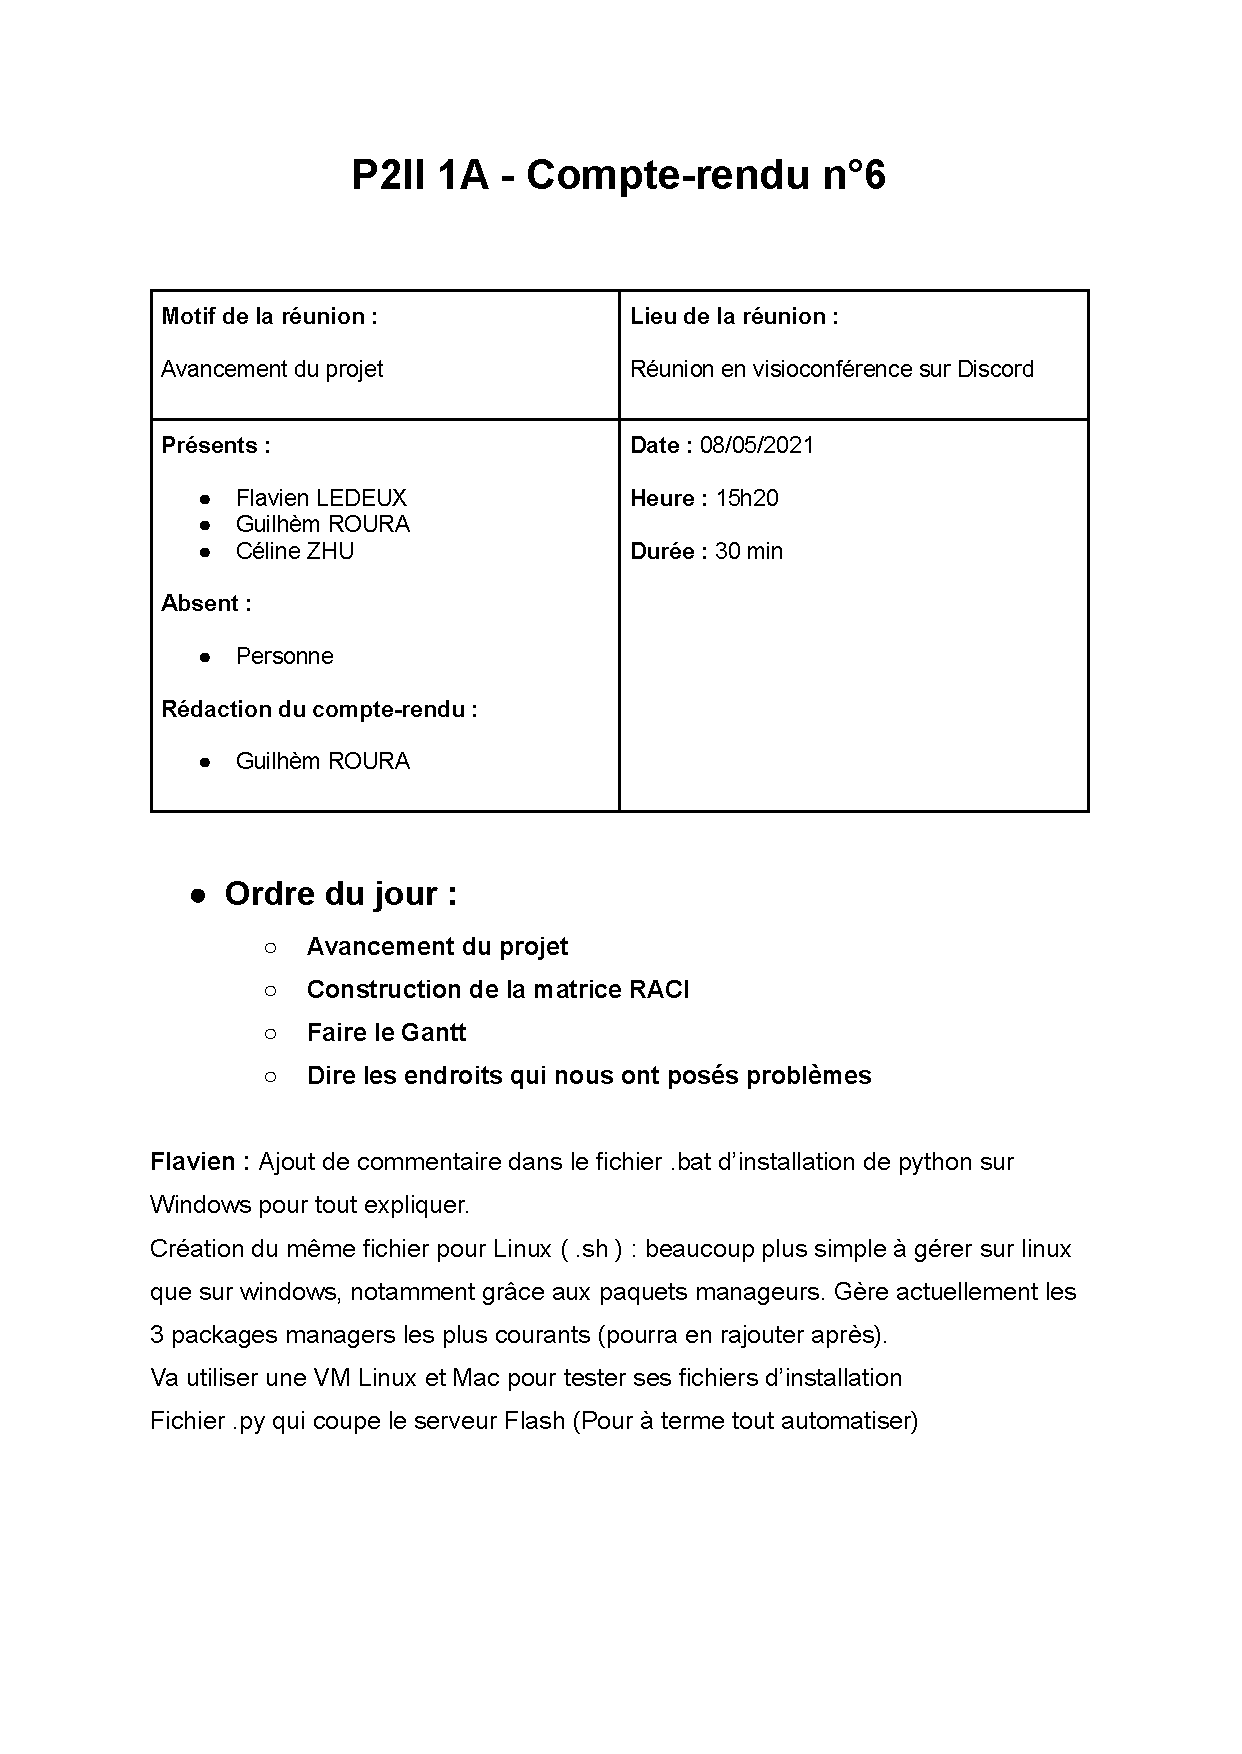
\includepdf[pages=-]{pdf/P2II_1A-Compte-rendu_n6.pdf}
\label{pdf:CR7}
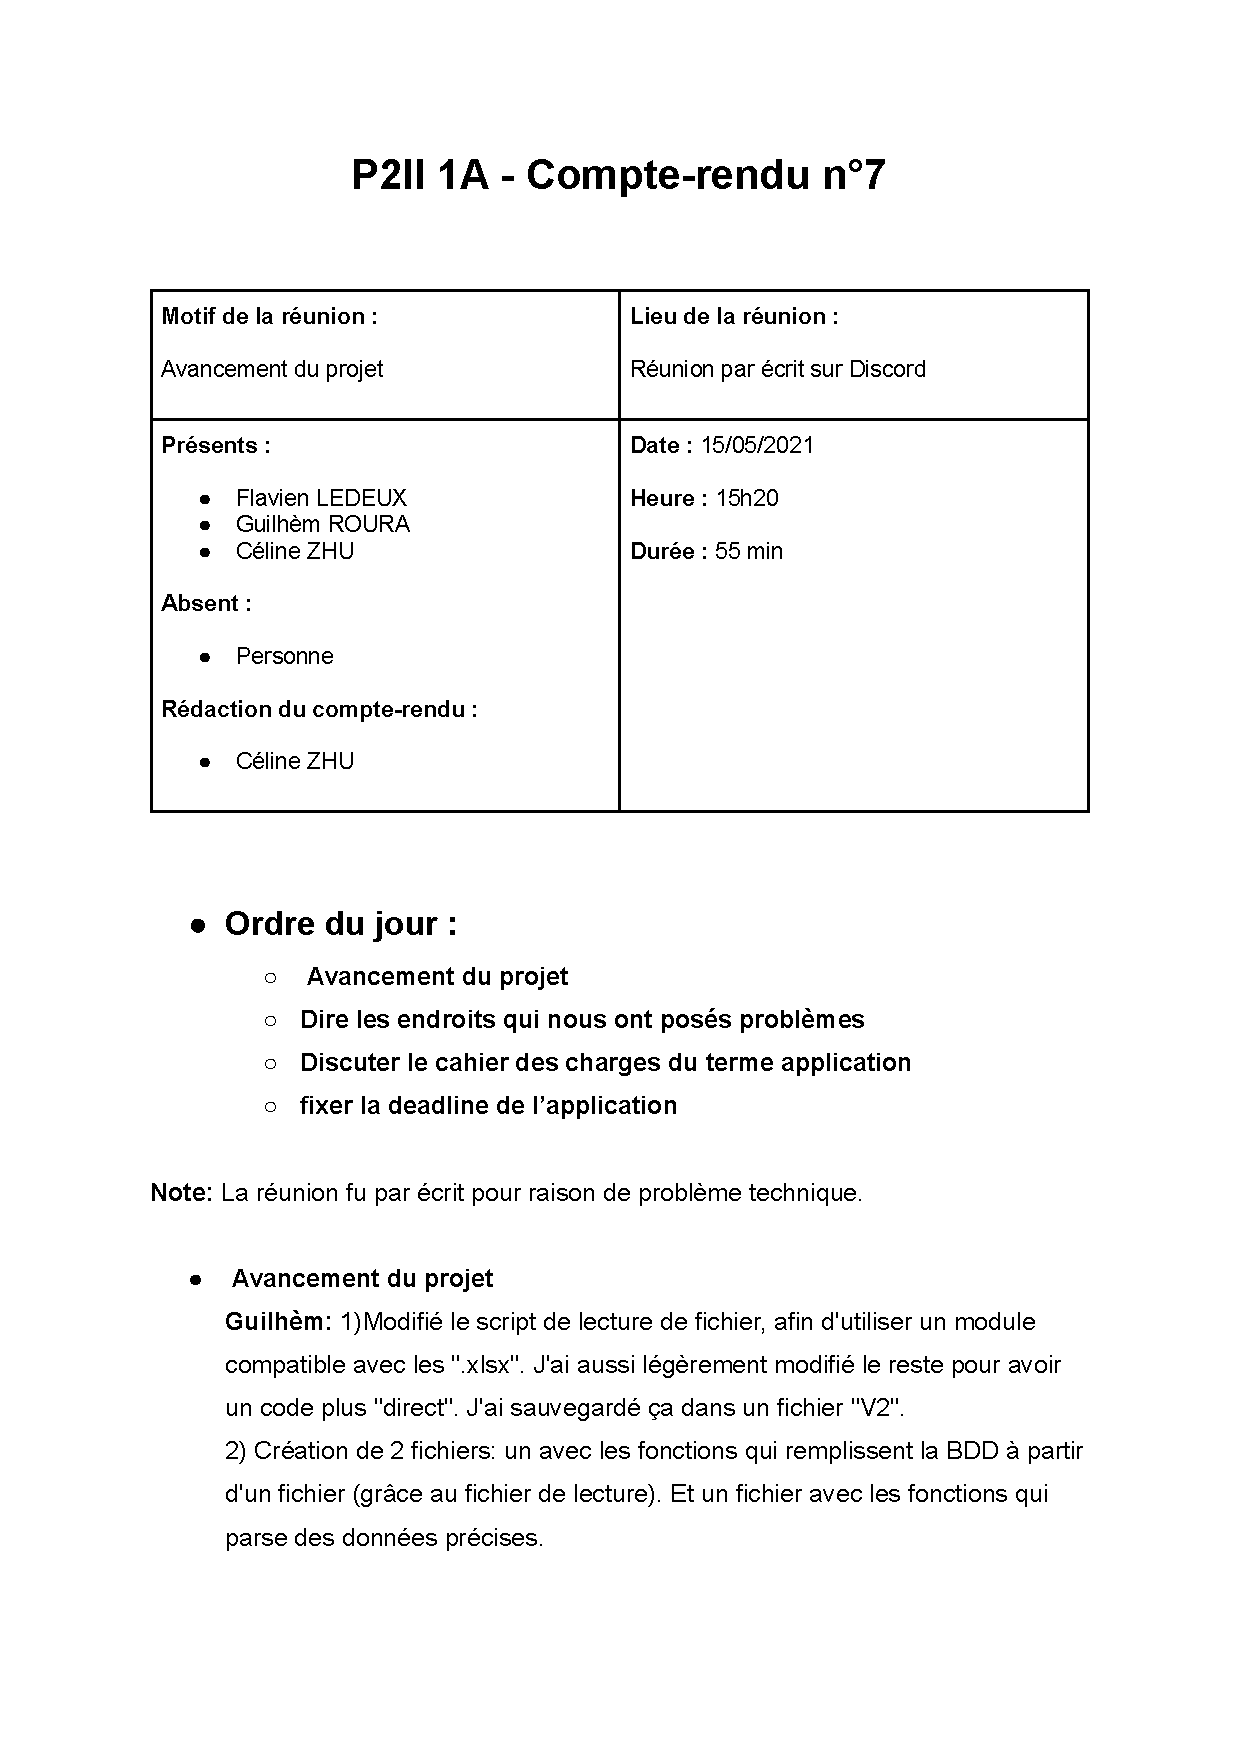
\includepdf[pages=-]{pdf/P2II_1A-Compte-rendu_n7.pdf}
\label{pdf:CR8}
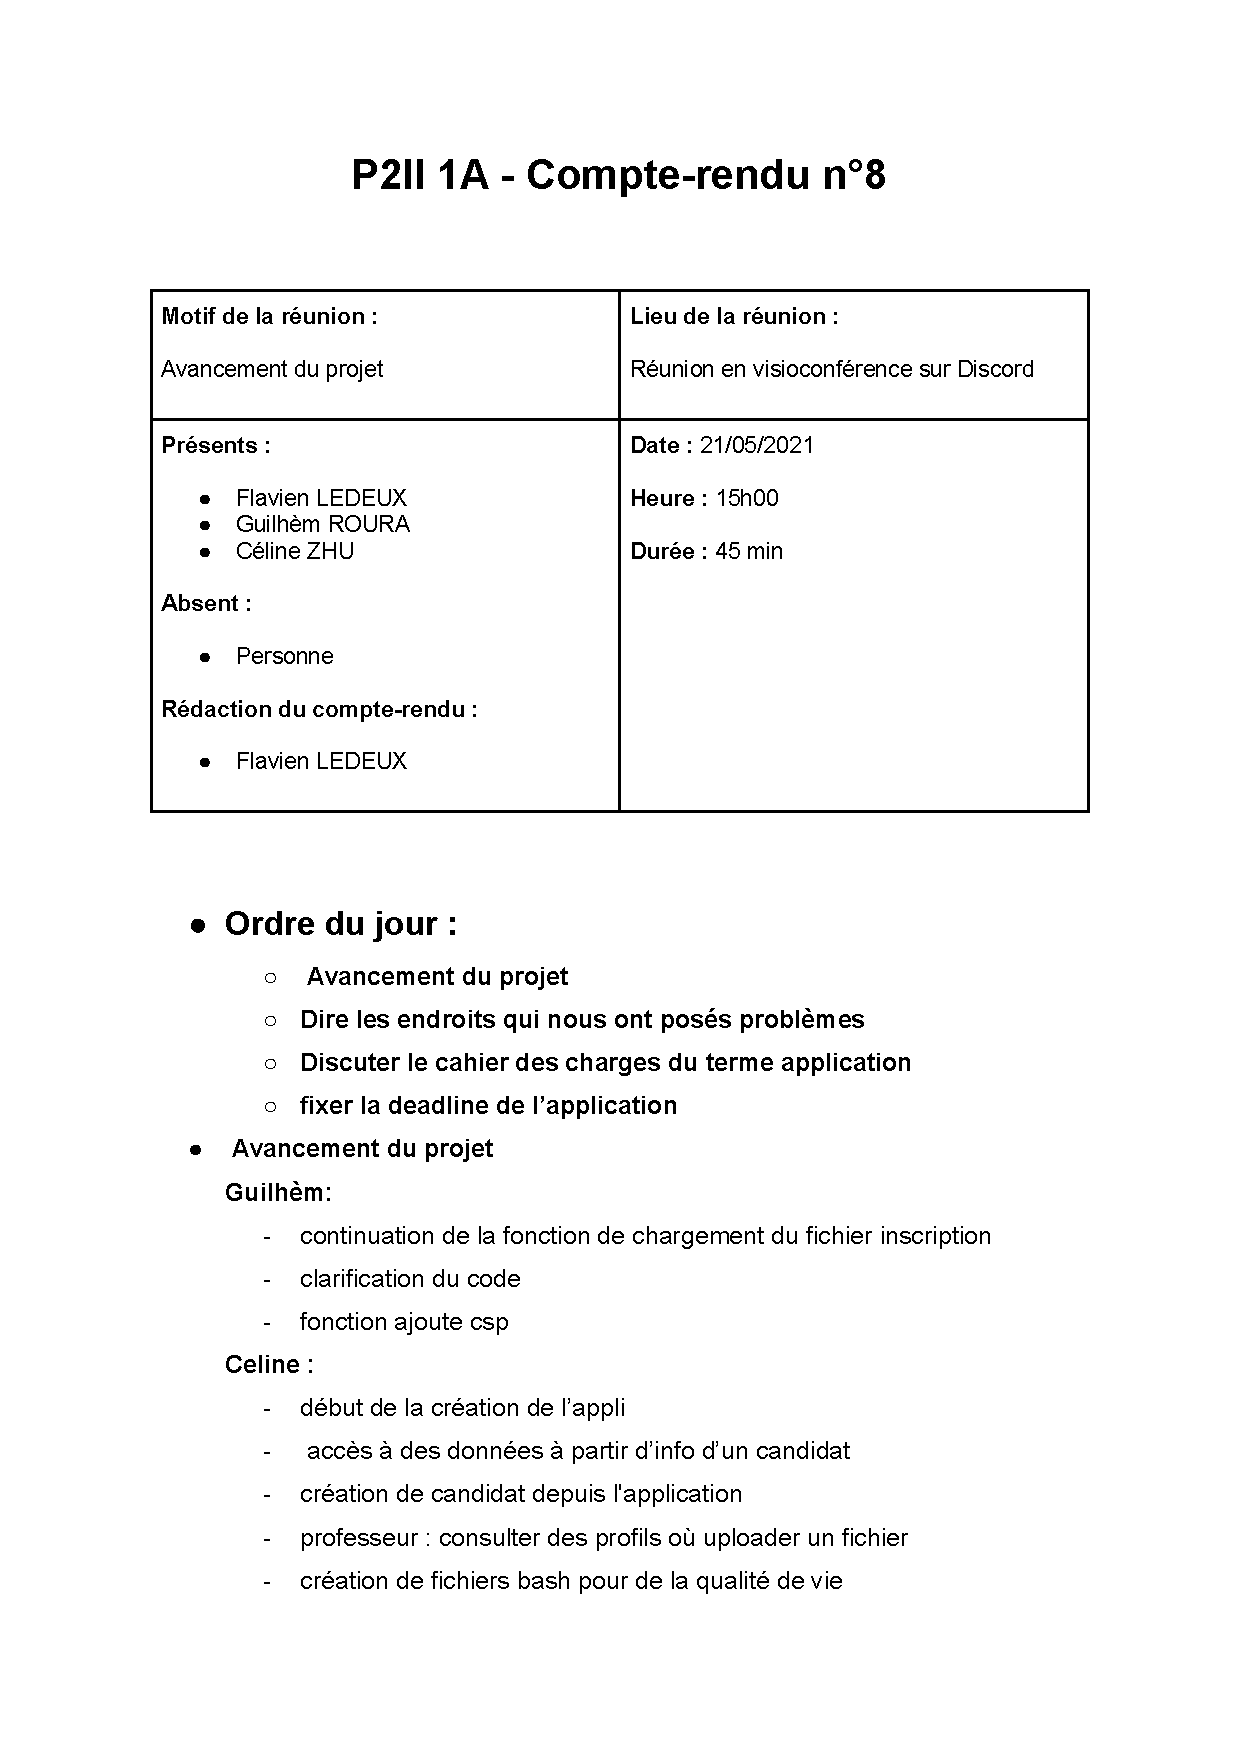
\includepdf[pages=-]{pdf/P2II_1A-Compte-rendu_n8.pdf}
\label{pdf:CR9}
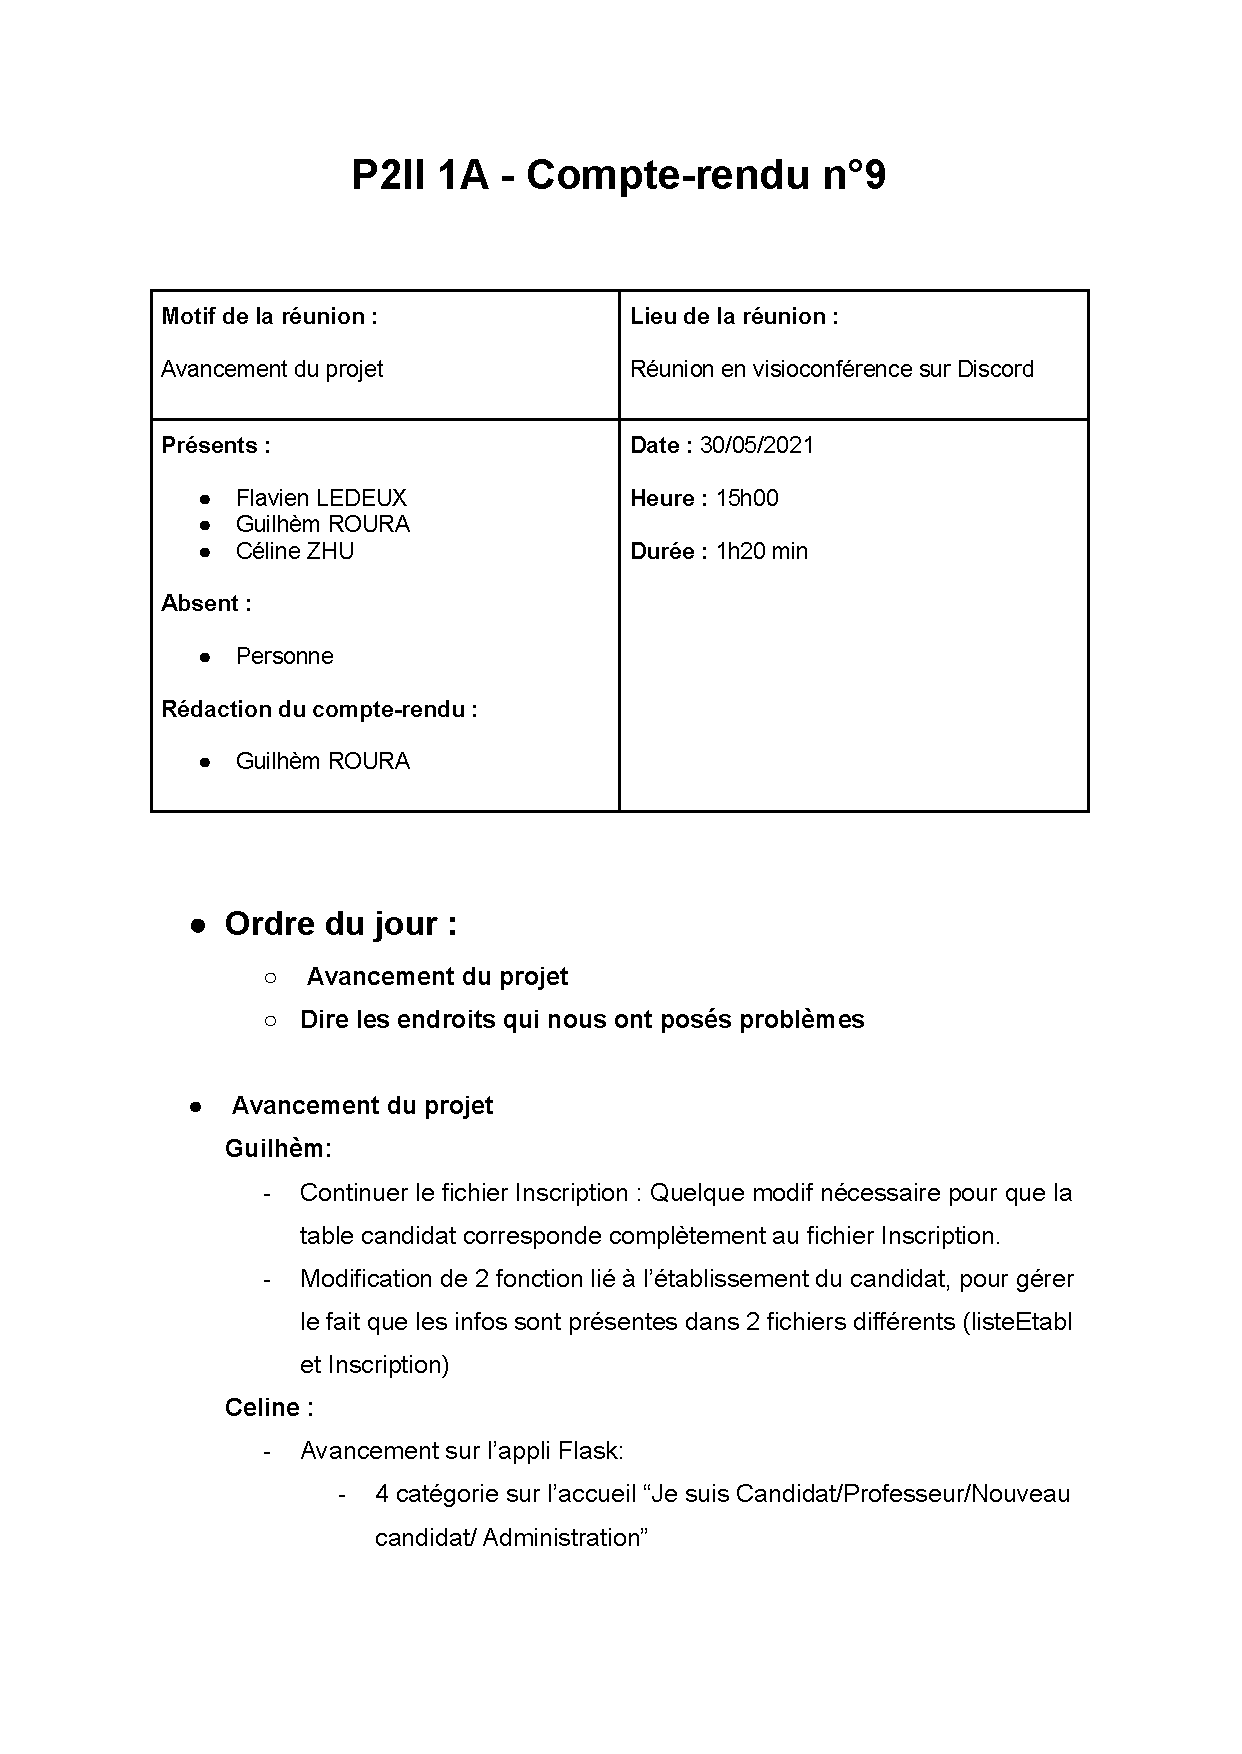
\includepdf[pages=-]{pdf/P2II_1A-Compte-rendu_n9.pdf}
\label{pdf:CR10}
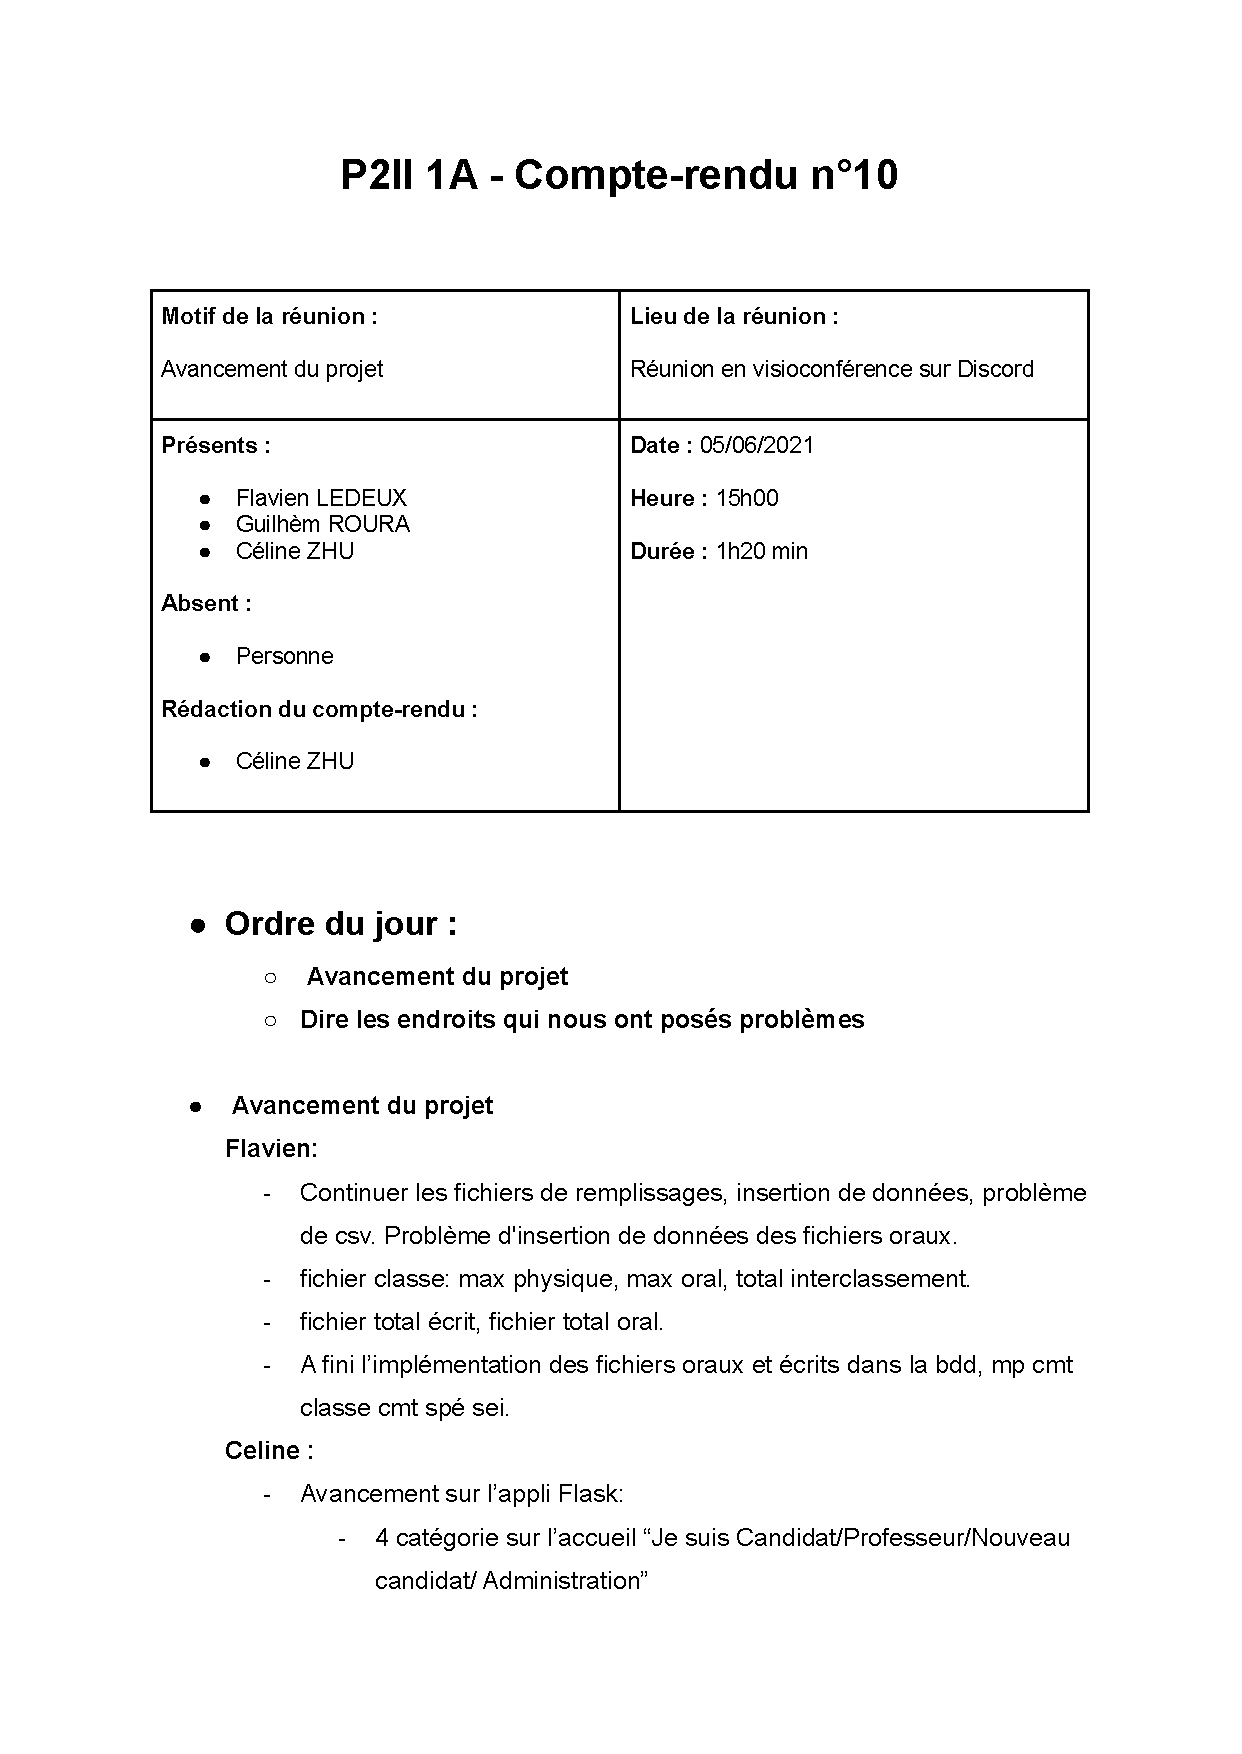
\includepdf[pages=-]{pdf/P2II_1A-Compte-rendu_n10.pdf}
\label{pdf:charte}
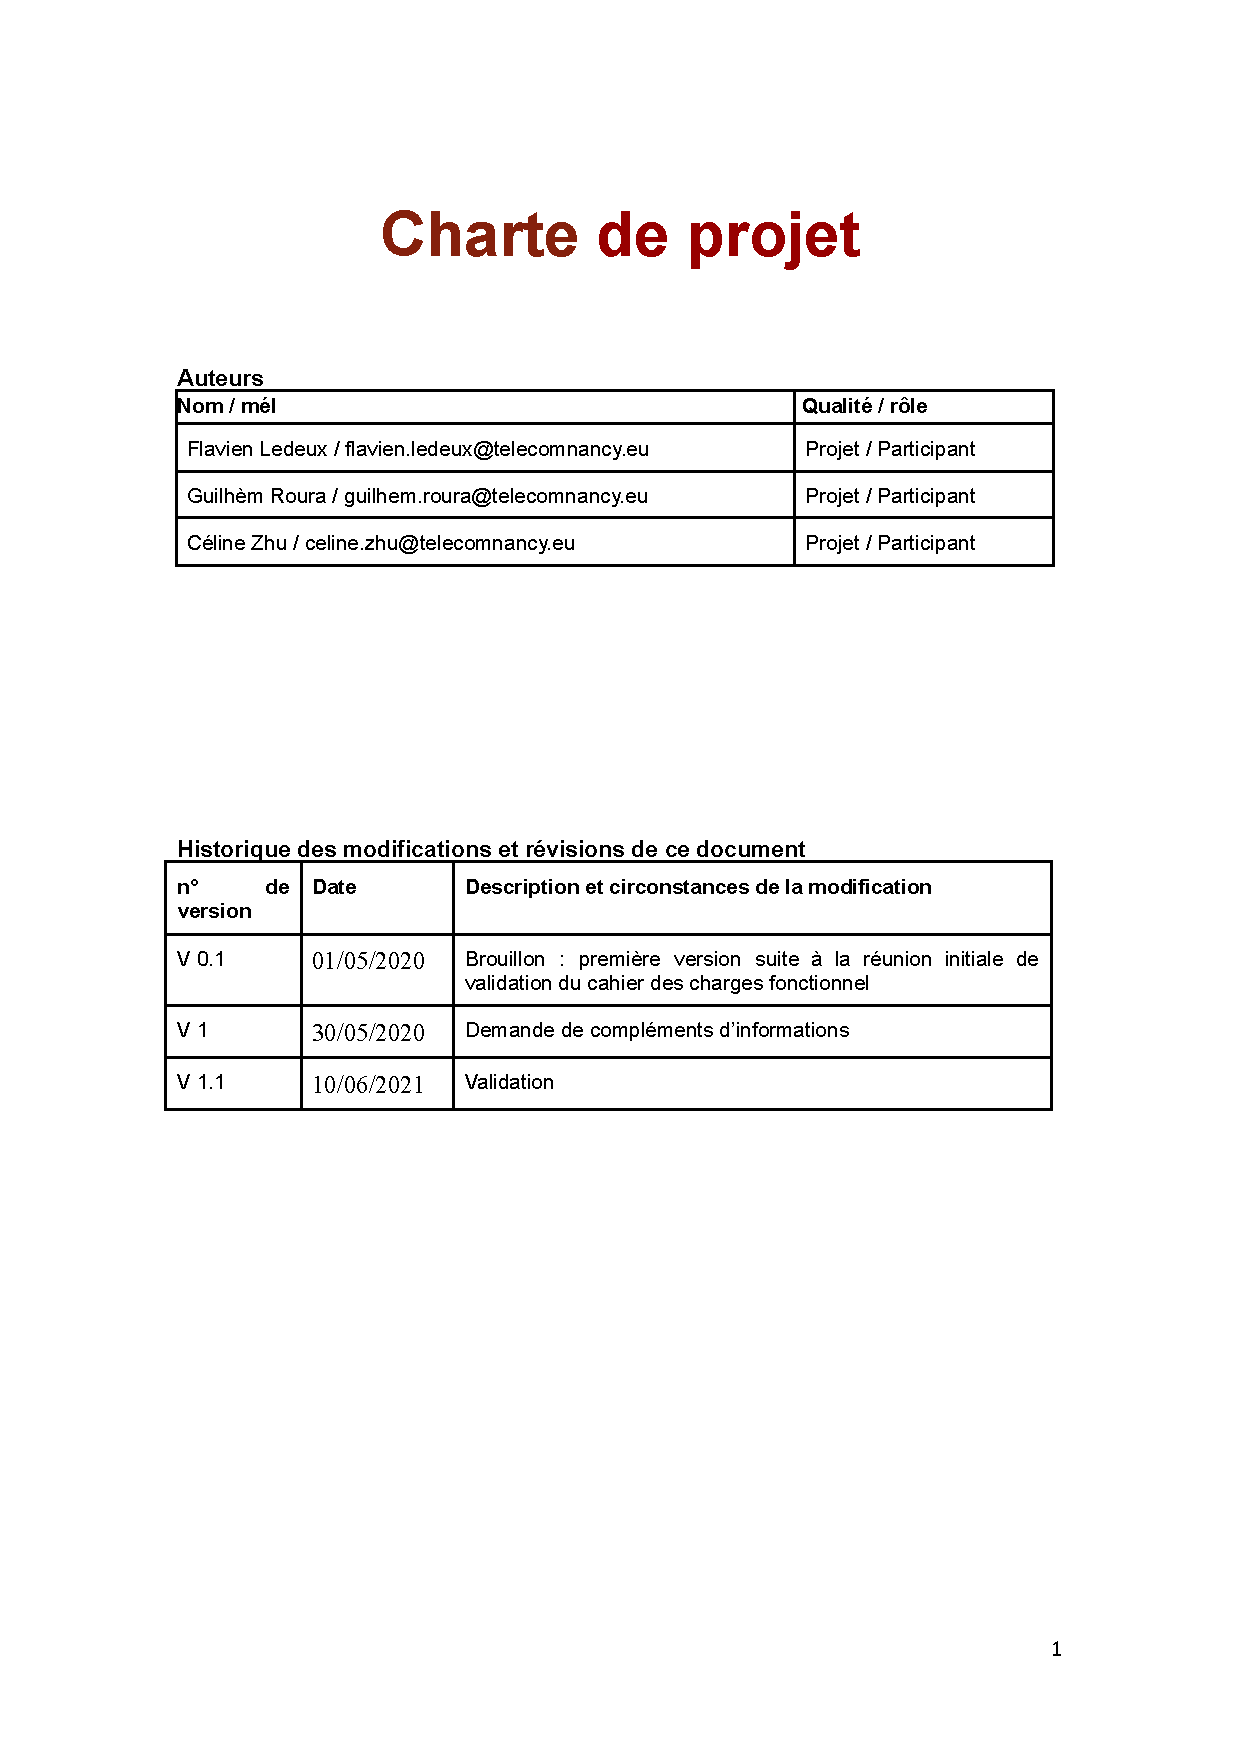
\includepdf[pages=-]{pdf/Charte_de_projet.pdf}
\label{pdf:installation}
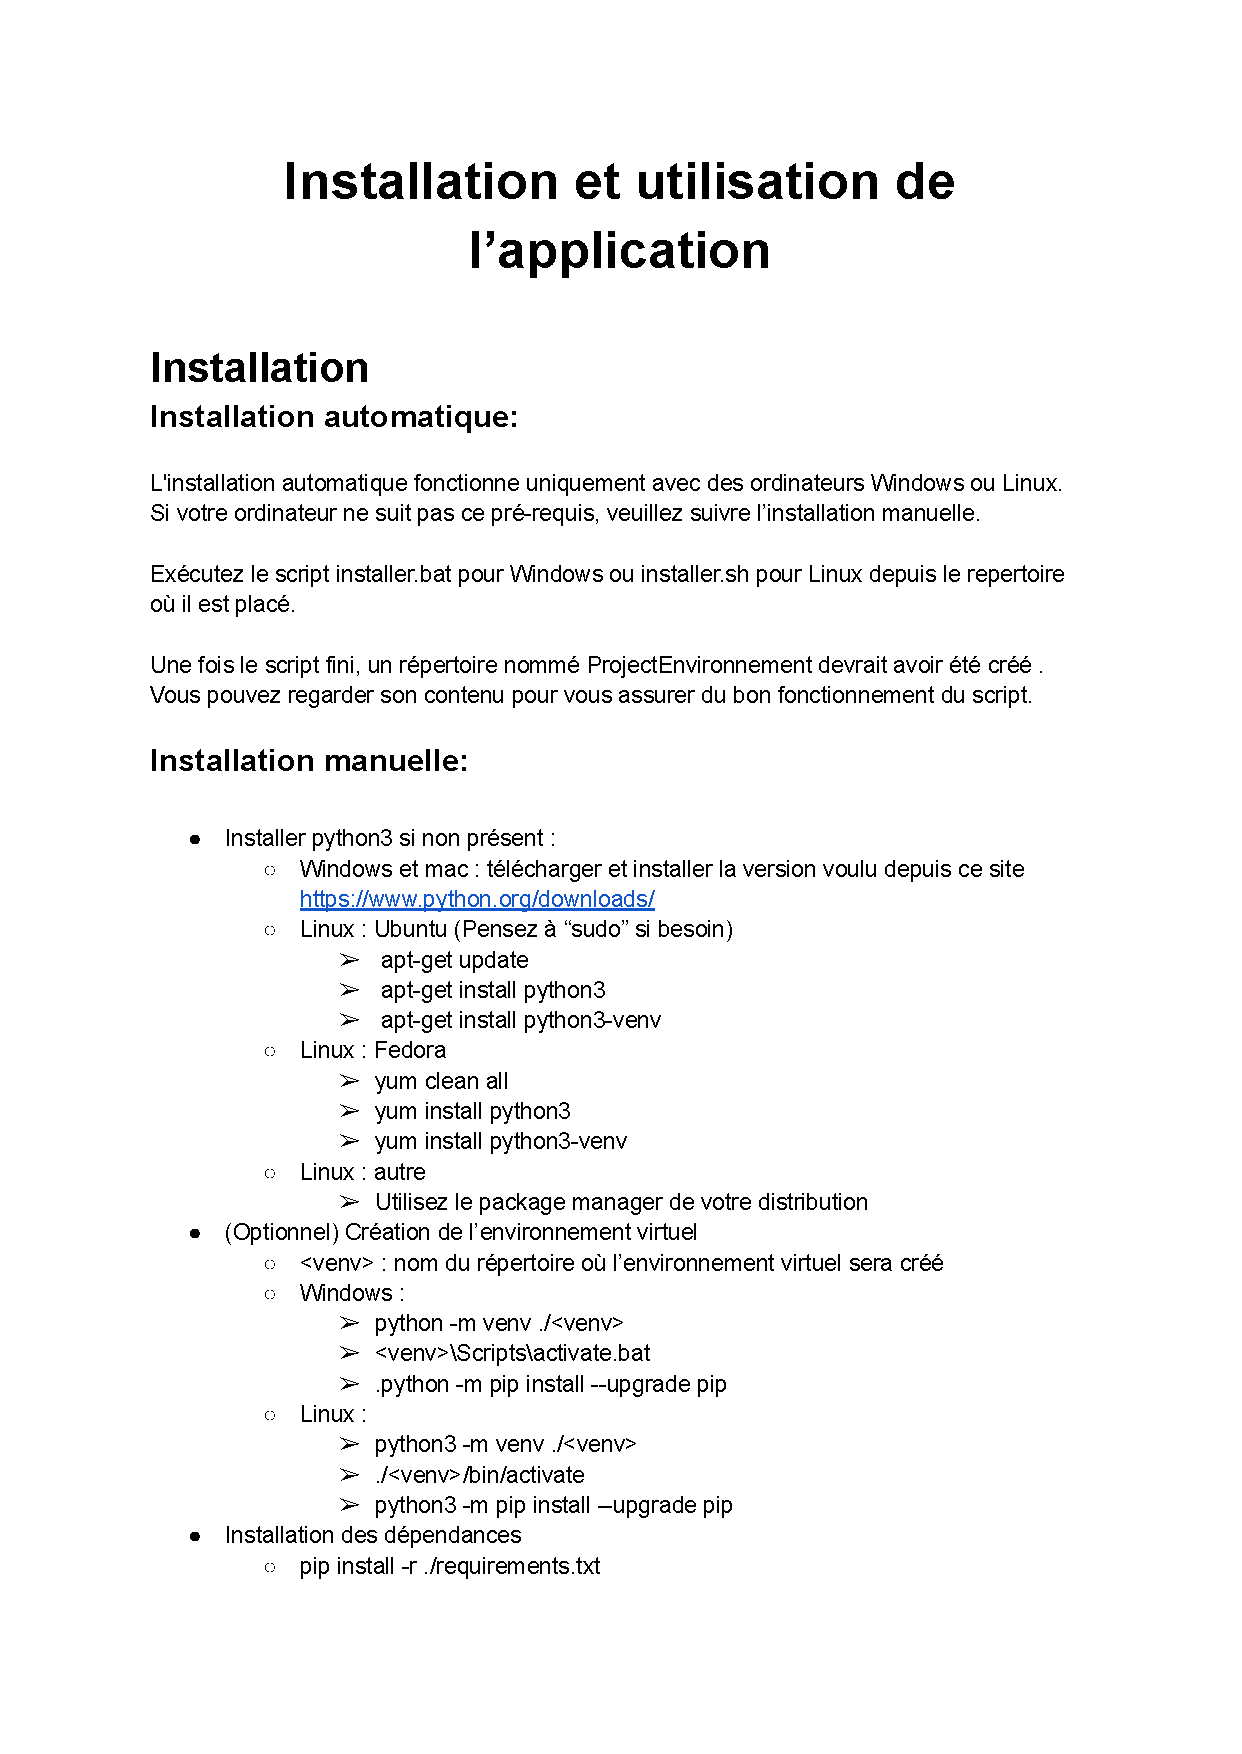
\includepdf[pages=-]{pdf/Manuel_d'installation.pdf}






\end{document} 